
\chapter{The role of trust in knowledge based communities} % Main chapter title
\label{ChapterTrust}

Information and communications technologies (ICTs) have enabled faster and easier creation and sharing of knowledge. Furthermore, they have provided access to a large amount of data which enabled a detailed study of their emergence and evolution \cite{dankulov2015dynamics}, as well as user's roles \cite{saxena2021users}, patterns of their activity \cite{santos2019activity, slag2015one, chhabra2020activity}. 
However, relatively small attention was given to sustainability of SE communities. Most of the research was focused on the activity and factors that influence the increase of the users’ activity in these communities. Factors such as need for experts and the quality of their contributions have been thoroughly investigated \cite{dev2018size}. It was shown that growth of communities and mechanisms that drive it may depend on the topic around which the community was created \cite{santos2019self}. \\

\section{The Stack Exchange}

The Stack Exchange is a network of question-answer websites on diverse topics. In the beginning, the focus was on computer programming questions with StackOverflow \footnote{
	More information about StackOverlflow is available at: \url{https://stackoverflow.co/} and broad introduction to StackExchange network is available at: \url{https://stackexchange.com/tour}. 
}  community. Its popularity led to the creation of the Stack Exchange network that these days counts more than 100 communities on different topics. The SE communities are self-moderating, and the questions and answers can be voted, allowing users to earn Stack Exchange reputation and privileges on the site. 

The new site topics are proposed through site Area51 \footnote{Visit \url{https://area51.stackexchange.com/faq} for more details about closed and beta SE communities and the review process.}, and if the community finds them relevant, they are created. Every proposed  StackExchange site needs interested users to commit to the community and contribute by posting questions, answers and comments. After a successful private beta phase site reaches the public beta phase, other members are allowed to join the community. The site can be in the public beta phase for a long time until it meets specific SE evaluation criteria for graduation. Otherwise, it may be closed with a decline in users' activity. 

We focused analysis on four pairs of SE communities with the same topic. Astronomy, Literature and Economics are active communities \footnote{Astronomy, Literature and Economics graduated on December 2021 and during our research, they were still in the public beta phase.} The first time, these communities were unsuccessful and thus closed. We also compare closed Theoretical Physics with the Physics site, considering that those two topics engage similar type of users.

\subsection{Data}
Stack Exchange data are public and regularly released. As closed communities were active between 180 and 210 days, we extracted only first 180 days of data. Given that first few months can be crucial for further development of the community \cite{dover2020sustainable}, we are interested in early evolution of Stack Exchange sites. 

Detailed information about questions, answers, and comments are available for each SE community. Each post is labelled with a unique ID, the user's ID who made the post, and creation time. On Stack Exchange, users interact on several layers: Those interactions are considered positive.
\begin{itemize}
	\item posting an answer on the question; for every question, we extract IDs of its answers
	\item posting a comment on the question or answer; for every question and answer, we selected IDs of its comments
	\item accepting answer; for each question, we selected the accepted answer ID
\end{itemize}

Even though posts can be voted and downvoted, information about a user who voted is absent, so we do not consider these interactions between users. Comments can not be downvoted, while we find only around 3\% negatively voted answers and questions, Table \ref{tab:negint}.

\begin{table}[hbt!]
	\centering
	\caption{Percentage of negatively voted interactions}
	\label{tab:negint}
	\begin{tabular}{cc|cc}

		\hline
		Site                        & Status & Questions & Answers \\ \hline
		\multirow{2}{*}{Physics}    & Beta   & 5\%       & 4\%     \\
		& Closed & 1\%       & 2\%     \\ \hline
		\multirow{2}{*}{Astronomy}  & Beta   & 3\%       & 3\%     \\
		& Closed & 2\%       & 1\%     \\ \hline
		\multirow{2}{*}{Economics}  & Beta   & 4\%       & 4\%     \\
		& Closed & 7\%       & 4\%     \\ \hline
		\multirow{2}{*}{Literature} & Beta   & 2\%       & 5\%     \\ 
		& Closed & 2\%       & 1\%     \\ \hline \hline
		\textbf{Average}            &        & 3.2\%     & 3\%     \\ \hline 
	\end{tabular}
\end{table}


%The data contains information about the official StackExchange reputation of each user but only as a single value measuring the final reputation of the user on a day when data archive was released. Because of this significant shortcoming, we do not include this information in our analysis. In SE users can give positive or negative votes to questions and answers, and mark questions as favor, however the data is again provided as a final score recorded at the moment of the realise of the database. Since this does not allows us to analyse the evolution of scores, we omit this data from our analysis.\\


\subsection{Comparison between active and closed SE communities}

Table \ref{tab:site-info} compares the first 180 days between closed and active communities. When it comes to basic statistics, active communities had larger number of users, questions, answers and comments. Another simple indicator if community is going to graduate or decline can be time series of active questions for period of 7 days in Figure \ref{fig:active_questions}. The question is active if had at least one activity, posted answer ot comment during previous seven days. We find that live communities have larger number of active questions after first three months. Still, this difference is smaller for literature and astronomy. For astronomy we observe that closed community had higher number of active questions in the early period of community life. \\~\\


\begin{table}[h]
	\centering
	\caption{Community overview for first 180 days, Number of users $n_u$, number of questions $n_q$, number of answers $n_a$, number of comments $n_c$}
	\label{tab:site-info}
	\begin{tabular}{llccccc}
		\toprule
		Site                 & Status                           & First Date                     & $n_u$                    & $n_q$                & $n_a$                  & $n_c$ \\ \hline
		\multirow{2}{*}{Astronomy}  & \multicolumn{1}{l|}{Closed}      & \multicolumn{1}{c|}{09/22/10} & \multicolumn{1}{c|}{336}  & \multicolumn{1}{c|}{474}  & \multicolumn{1}{c|}{953}  & 1444     \\
		& \multicolumn{1}{l|}{Beta} & \multicolumn{1}{c|}{09/24/13} & \multicolumn{1}{c|}{405}  & \multicolumn{1}{c|}{644}  & \multicolumn{1}{c|}{959}  & 2170     \\ \hline
		\multirow{2}{*}{Economics}  & \multicolumn{1}{l|}{Closed}      & \multicolumn{1}{c|}{10/11/10} & \multicolumn{1}{c|}{275}  & \multicolumn{1}{c|}{368}  & \multicolumn{1}{c|}{458}  & 1253     \\
		& \multicolumn{1}{l|}{Beta} & \multicolumn{1}{c|}{11/18/14} & \multicolumn{1}{c|}{648}  & \multicolumn{1}{c|}{1024} & \multicolumn{1}{c|}{1410} & 3553     \\ \hline
		\multirow{2}{*}{Literature} & \multicolumn{1}{l|}{Closed}      & \multicolumn{1}{c|}{02/10/10} & \multicolumn{1}{c|}{284}  & \multicolumn{1}{c|}{318}  & \multicolumn{1}{c|}{523}  & 1097     \\
		& \multicolumn{1}{l|}{Beta} & \multicolumn{1}{c|}{01/18/17} & \multicolumn{1}{c|}{478}  & \multicolumn{1}{c|}{910}  & \multicolumn{1}{c|}{907}  & 3301     \\ \hline
		\multirow{2}{*}{Physics}    & \multicolumn{1}{l|}{Closed}      & \multicolumn{1}{c|}{09/14/11} & \multicolumn{1}{c|}{281}  & \multicolumn{1}{c|}{349}  & \multicolumn{1}{c|}{564}  & 2213     \\
		& \multicolumn{1}{l|}{Launched}    & \multicolumn{1}{c|}{08/24/10} & \multicolumn{1}{c|}{1176} & \multicolumn{1}{c|}{2124} & \multicolumn{1}{c|}{4802} & 15403    \\
		\bottomrule \\~\\
	\end{tabular}
\end{table}


\begin{figure}
	\centering
	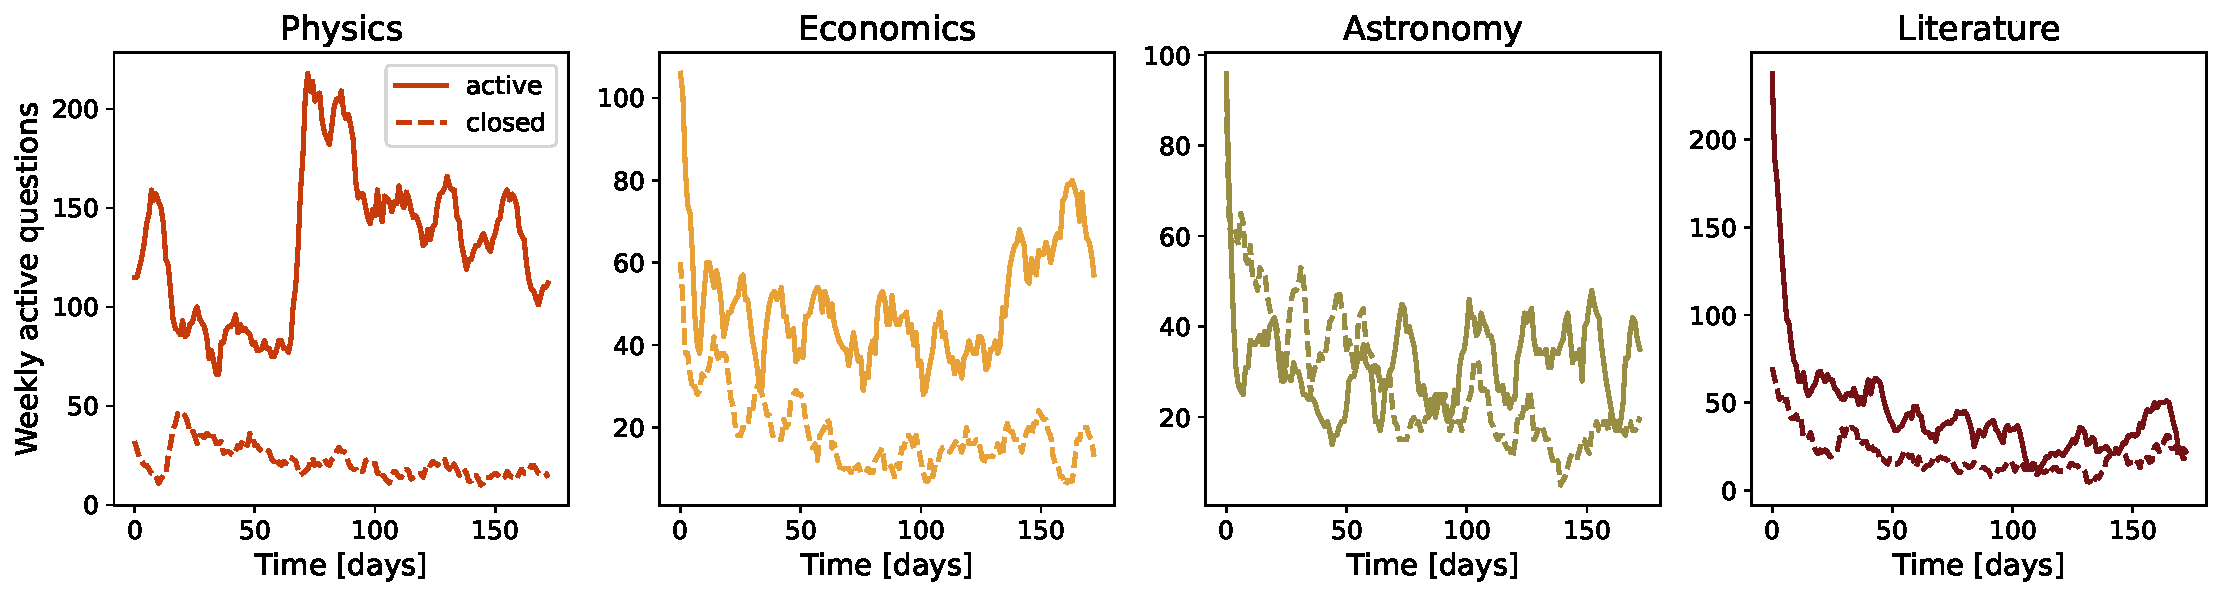
\includegraphics[width=\linewidth]{figures/stackexchange/active_questions.pdf}
	\caption{Number of active questions within 7 days sliding windows. Solid line - active sites; dashed lines - closed sites.}
	\label{fig:active_questions}
\end{figure}

Similarly, the official Stack Exchange community evaluation process considers simple metrics \footnote{\href{https://stackoverflow.blog/2011/07/27/does-this-site-have-a-chance-of-succeeding/}{https://stackoverflow.blog/2011/07/27/does-this-site-have-a-chance-of-succeeding/}}. To determine the the success of sites  they measure how many questions are answered, how many questions are posted per day, and how many answers are posted per question.  There are two measures: the number of avid users and the number of visits that are not easily interpreted from the data. The site is \textit{healthy} if it has 10 questions per day, 2.5 answers per question and more than $90\%$ of answered questions. For less than $80\%$ of answered questions, 5 questions per day and 1 question per answer site \textit{needs some work}. 

We calculated Stack Exchange statistics for astronomy, economics, literature and physics and results are presented in the Table \ref{tab:se_c}. After observed period of 180 days only live physics is healthy site while other live communities are at least in two criteria labeled as \textit{okay}. Closed sites mostly \textit{need some work}, the exception is closed astronomy. For example it has \textit{excellent} percent of answered questions and \textit{okay} answer ratio.  

%While Physics community was clearly more successful than Theoretical Physics and other considered communities, we see that these differences are not as clear if we compare three other pairs of communities. For instance, some of the parameters for closed Astronomy community were better than for the community that is still alive. Similar results were found for Economics and Literature. 

\begin{table}[h!]
	%\footnotesize\sf\centering
	\caption{Community overview for first 180 days according to SE criteria  }
	
	\label{tab:se_c}
	\begin{tabular}{ccccc}
		\hline
		
		Site & Status &  Answered & Questions per day & Answer ratio \\ \hline
		\multirow{2}{*}{Astronomy} & \multicolumn{1}{c|}{Closed} & \multicolumn{1}{c|}{\textbf{95} \%}  & \multicolumn{1}{c|}{2.62} & \multicolumn{1}{c}{\underline{2.02}} \\
		& \multicolumn{1}{c|}{Beta} & \multicolumn{1}{c|}{\textbf{96} \%}  & \multicolumn{1}{c|}{3.57} & \multicolumn{1}{c}{\underline{1.49}} \\ \hline
		\multirow{2}{*}{Economics} & \multicolumn{1}{c|}{Closed} & \multicolumn{1}{c|}{68 \%}  & \multicolumn{1}{c|}{2.04} & \multicolumn{1}{c}{\underline{1.25}} \\
		& \multicolumn{1}{c|}{Beta} & \multicolumn{1}{c|}{\underline{84} \%}  & \multicolumn{1}{c|}{\underline{5.66}} & \multicolumn{1}{c}{\underline{1.37}} \\ \hline
		\multirow{2}{*}{Literature} & \multicolumn{1}{c|}{Closed} & \multicolumn{1}{c|}{79 \%}  & \multicolumn{1}{c|}{1.77} & \multicolumn{1}{c}{\underline{1.65}} \\
		& \multicolumn{1}{c|}{Beta} & \multicolumn{1}{c|}{74 \%}  & \multicolumn{1}{c|}{\underline{5.04}} & \multicolumn{1}{c}{\underline{1.10}} \\ \hline
		\multirow{2}{*}{Physics} & \multicolumn{1}{c|}{Closed} & \multicolumn{1}{c|}{83 \%}  & \multicolumn{1}{c|}{1.93} & \multicolumn{1}{c}{\underline{1.64}} \\
		& \multicolumn{1}{c|}{Beta} & \multicolumn{1}{c|}{\textbf{93} \%}  & \multicolumn{1}{c|}{\textbf{11.76}} & \multicolumn{1}{c}{ \textbf{2.74}} \\ \hline \hline
		{Stack Exchange criteria} & excellent & $>$ 90 \% & $>$10 & $>$ 2.5   \\
		& needs some work & $<$ 80 \% & $<5$ & $<$ 1   \\ \hline
		
		
	\end{tabular}
	
\end{table}

This simple measurements presented in tables \ref{tab:site-info} and \ref{tab:se_c} and in figure \ref{fig:active_questions} do not provide us clear indications about community sustainability. Only for physics topic the difference between active and closed community is evident, while for other communities it is not so clear. Thus, we need deeper insights into structure and dynamics of these communities to understand. The structure of social interactions within communities and dynamics of collective trust may provide better explanation why some communities succeed and other died. 

\section{Network properties of Stack Exchange data}

On Stack Exchange sites, the interaction between users happens through posts. As we are interested in examining the characteristics of the users, we map interaction data to the networks. Using complex network theory, we can quantify the properties of obtained networks and compare different SE communities, e.g. alive and closed SE sites. 
In the user interaction network, the link between two nodes, user $i$ and $j$, exists if user $i$ answers or comments on the question posted by user $j$, or user $i$ comments on the answer posted by user $j$. The created network is undirected and unweighted, meaning that we do not consider multiply interactions between users or the direction of the interaction. 


\begin{figure}[h]
	\centering
	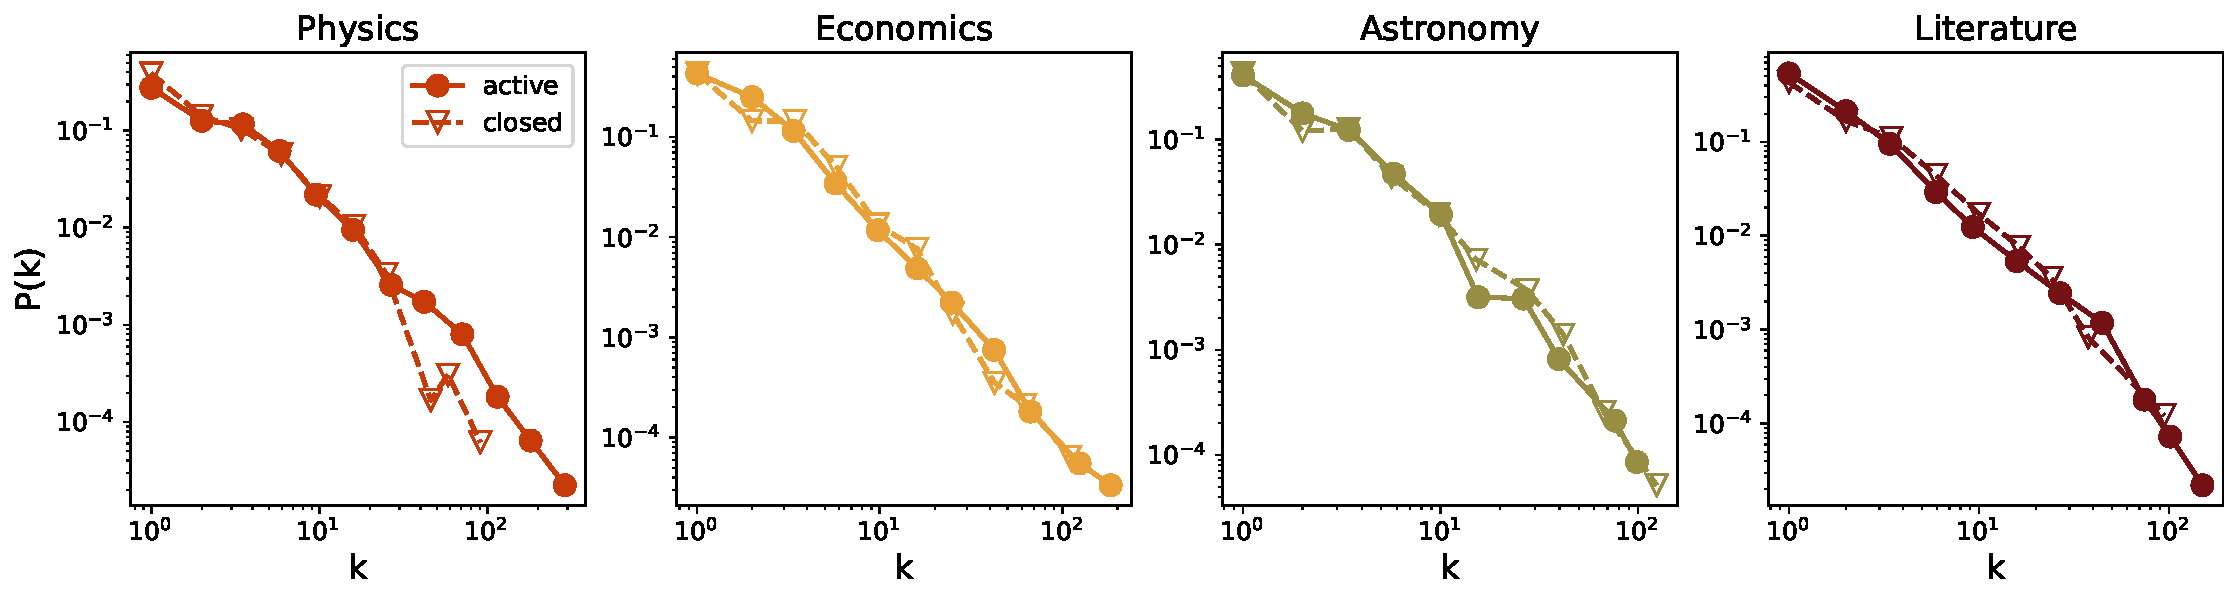
\includegraphics[width=\linewidth]{figures/stackexchange/degree_distribution_fullnet.pdf}%Figures/figures_SE/Fig3.pdf}
	\caption{Degree distribution.}
	\label{fig:fullnetdeg}
\end{figure}

\begin{figure}[h]
	\centering
	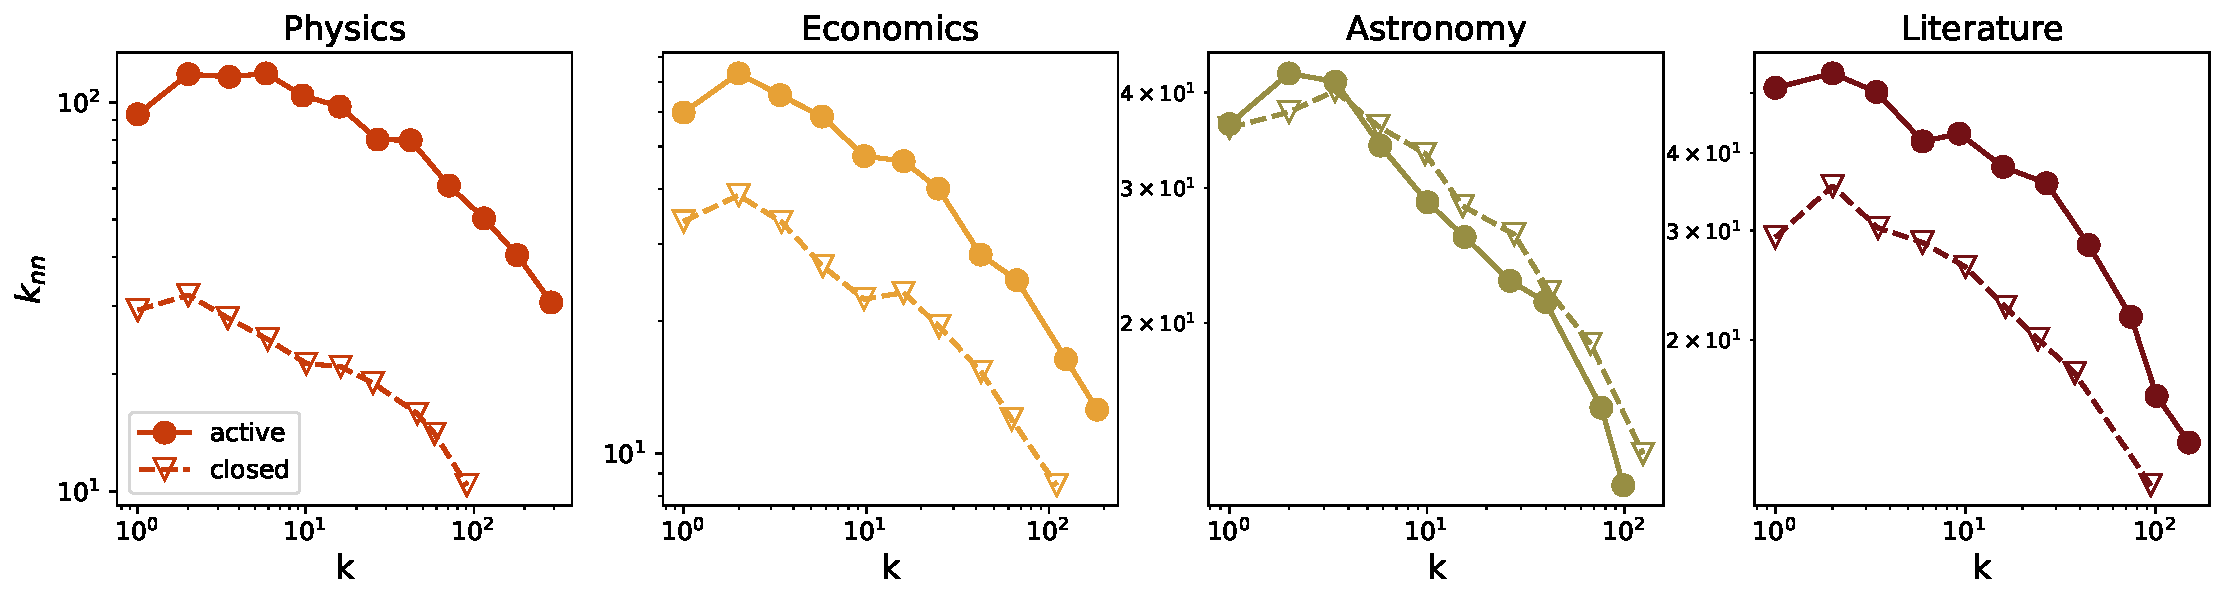
\includegraphics[width=\linewidth]{figures/stackexchange/neighdeg_fullnet.pdf}%Figures/figures_SE/Fig3.pdf}
	\caption{Neighbour degree.}
	\label{fig:fullneighdeg}
\end{figure}

\begin{figure}[h]
	\centering
	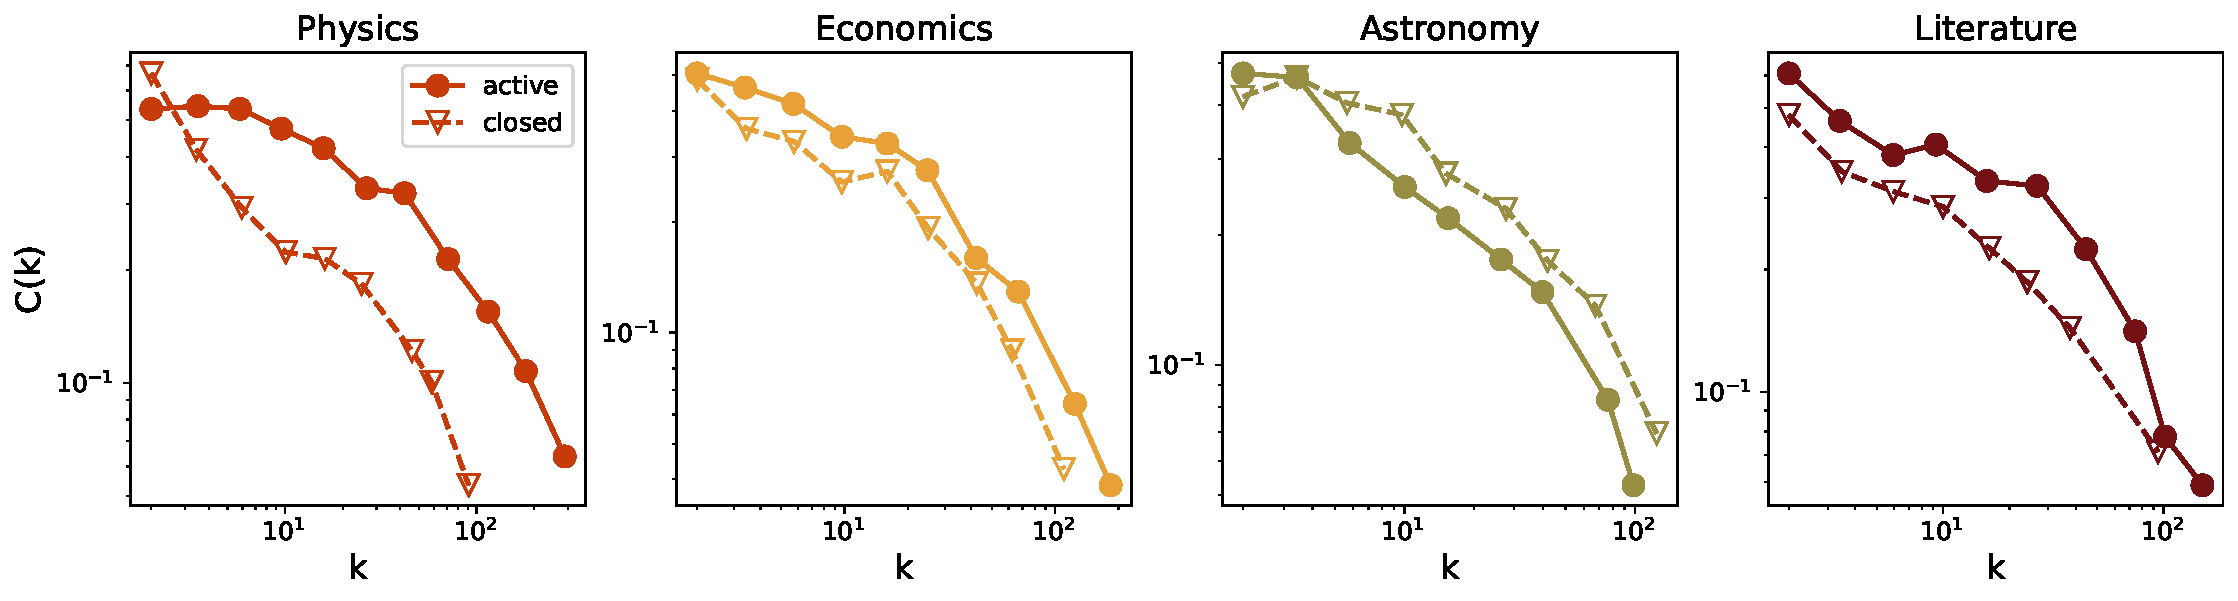
\includegraphics[width=\linewidth]{figures/stackexchange/clustering_fullnet.pdf}%Figures/figures_SE/Fig3.pdf}
	\caption{Neighbour degree.}
	\label{fig:fullneighdeg}
\end{figure}




Instead of creating a static network from the data in the first 180 days of community life, we study how network snapshots evolve. At each time step $t$, we create network snapshot $G(t, t+\tau)$, for time window of the length $\tau$. We fix the time window to $\tau=30$ days and slide it by $t=1$ day through time. Discussion of how the length of the sliding window influences the results is given in appendix A. Sliding the time window by one day, we can capture changes in the network structure daily, as two 30 days consecutive networks overlap significantly. 

We calculate different structural properties of observed networks and study their evolution. There are many local and global measures of the network properties \cite{boccaletti2006complex}. They are also dependent, still it was shown that degree distribution, degree-degree correlations and clustering coefficient can describe the properties of the most complex networks \cite{orsini2015quantifying}. 


%TODO degree distribution
%TODO degree correlations
%TODO clustering  




\subsection{Clustering}
The clustering coefficient of a node quantifies the average connectivity of between its neighbours and cohesion of its neighbourhood \cite{boccaletti2006complex}. It is a probability that two neighbours of a node are also neighbours, and is calculated using the following formula:
\begin{equation}
	c_{i}=\frac{e_{i}}{\frac{1}{2}k_{i}(k_{1}-1)} \ .
	\label{eq:clust}
\end{equation}
Here $e_{i}$ is the number of links between neighbours of the node $i$ in a network, while $\frac{1}{2}k_{i}(k_{i}-1)$ is the maximal possible number of links determined by the node degree $k_{i}$. The clustering coefficient of network $C$ is the value of clustering averaged over all nodes. Here we investigate how clustering coefficient in a SE community is changing with time by calculating its value for all network snapshots. We compare the behavior of clustering for active and closed communities on the same topic in order to better understand how cohesion of these communities is changing over time. 
Members' clustering coefficient measures the probability that other members connected to them are also connected. Study on dynamics of social group growth shows that that links between one's friends that are members of a social group increase the probability that that individual will join the social group \cite{backstrom2006group}. Furthermore, successful social diffusion  typically occur in networks with high value of clustering coefficient \cite{centola2007cascade}. These results suggest that high local cohesion should be a characteristic of sustainable communities.

We first analyse structural properties of Stack Exchange communities and examine the difference between successful and unsuccessful ones. We calculate the mean clustering coefficient for 30-days window networks and examine how it changes with time. Figure \ref{fig:clustering} shows the evolution of mean clustering coefficient for all eight communities. All communities that are still alive are clustered, with the value of mean clustering coefficient higher than 0.1. Physics, the only launched community, has the value of clustering coefficient above 0.2 for the first 180 days.
During larger part of the observed period, the clustering coefficient of an active community is higher compared to the clustering coefficient of its closed pair. If we compare active communities with their closed counterpart, the closed communities have higher value of the mean clustering coefficient in the early phase while later communities that are still active have higher values of clustering coefficient. These results suggest that all communities have relatively high local cohesiveness, and that lower values of clustering coefficient in the later phase of community life may be an indicator of its decline. 

\begin{figure}
	\centering
	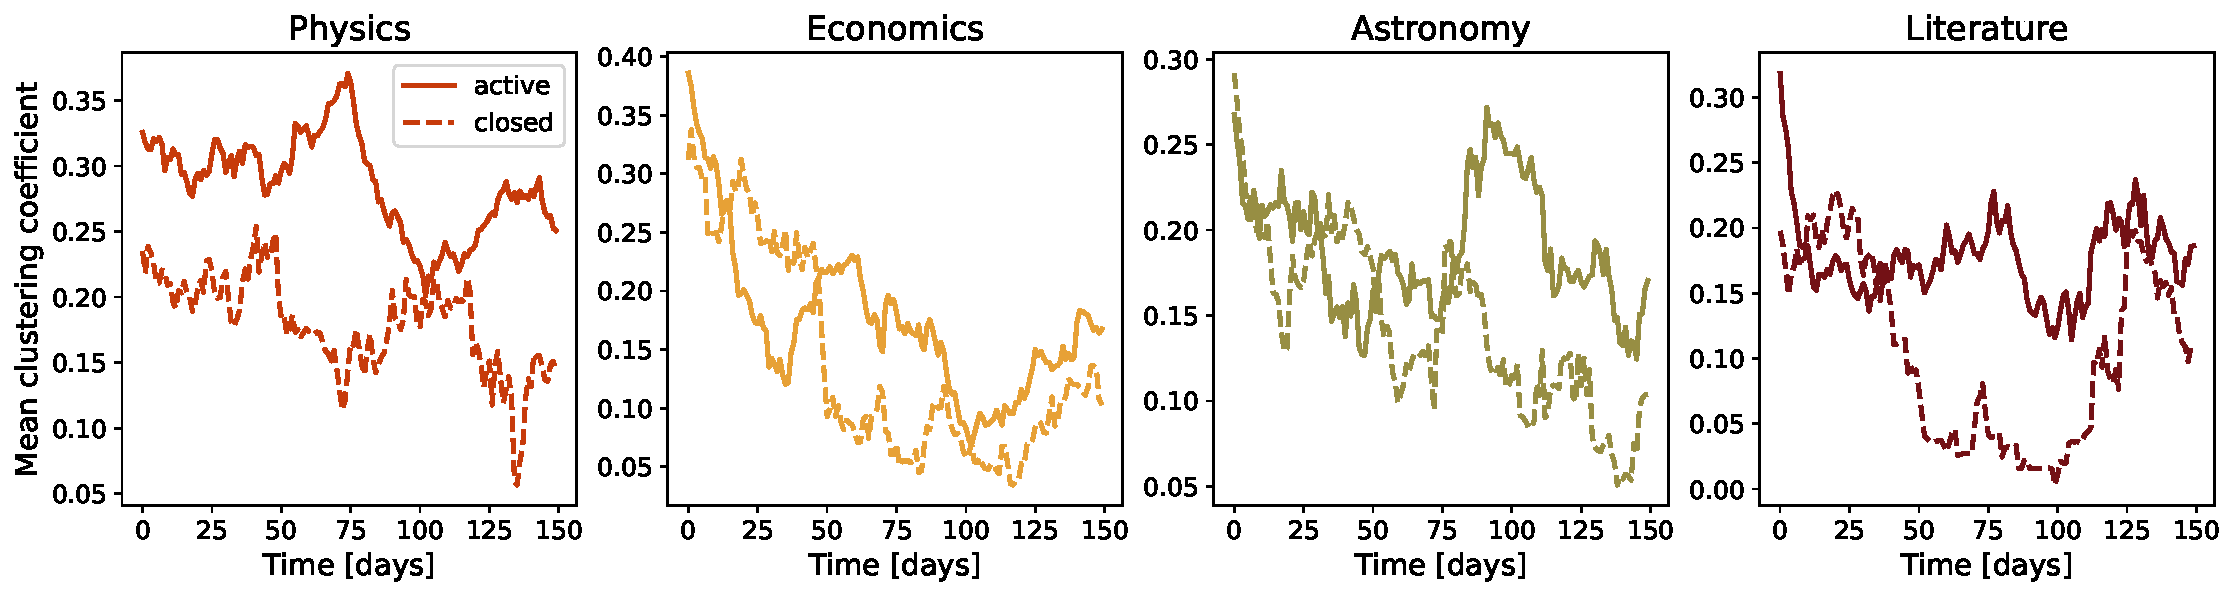
\includegraphics[width=\linewidth]{figures/stackexchange/clustering.pdf}%Figures/figures_SE/Fig3.pdf}
	\caption{Mean clustering coefficient.}
	\label{fig:clustering}
\end{figure}

\subsection{Core-periphery structure}

Real networks, including social networks, have a distinct mesocopic structure \cite{fortunato2010community, gallagher2020clarified}. Mescoscopic structure is manifested either through community structure or core-periphery structure. Networks that have community structure consist of a certain number of group of nodes that are densely connected with each other, with sparse connections between groups. Networks with core-periphery structure consist of two groups of nodes, with higher edge density within one group and between groups but low edge density in the second group \cite{gallagher2020clarified}. Research on dynamics of user interaction in SE communities shows that there is a small group of highly active members, similar to core,  that have frequent interactions with casual or low active members of community \cite{santos2019activity, santos2019self}. These results indicate that we should expect a core-periphery structure in SE communities. 

Core-periphery pattern means that network consists of two components: a core, densely connected group of nodes, and periphery, a second group of nodes that are loosely connected with the core and with each other. Classification of nodes into one of these two groups provide us with information about their functional and dynamical roles in the network. Active users typically belong to core, while periphery consists of less active users.

To investigate core-periphery structure of SE communities and how it evolves trough time, we analyse the core-periphery structure of every 30 days network snapshot. We use Stochastic Block Model (SBM) adapted for core-periphery inference of network structure \cite{gallagher2020clarified} to determine the core-periphery structure.  

%\subsection{Core-periphery sample}
For each 30 days snapshot network we run 50 iterations and choose the model parameters $\theta$ and $p$ according to minimum description length. MDL does not change much among inferred core-periphery structure, see Fig. A8, while looking into adjusted rand index we can notice that difference exists. Still, ARI between pair-wised compared partitions is large ($ari >0.9$) indicating stability of inferred structures.

\subsection{core-periphery structure of knowledge-sharing networks}

Furthermore, we examine core-periphery structure of these communities and its evolution. Specifically, we are interested in the evolution of connectivity in the core. Figure \ref{fig:links_per_node} shows the number of links between nodes in the core per node $\frac{L}{N}(t)$. $\frac{2L}{N}$ is the average degree of the node in the core, and thus, $\frac{L}{N}$ is the half of the average degree. Again, Physics community has the much higher value of this quantity than Theoretical physics during the whole observed period, indicating higher connectivity between core members. Higher connectivity between core members in the active community is also characteristic for Literature, although this quantity has the same value for active and closed communities at the end of the observation period. The differences between active and closed communities are not that evident for Economics and Astronomy, see Fig. \ref{fig:links_per_node}. Active and closed Economics communities have similar connectivity in the core during the first 50 days. After this period, the connectivity in the core of the active community the twice as large as in the closed community and the difference grows at the end of observation period. The connectivity in the core of closed Astronomy community is higher that the connectivity in the core of the active community during the first 50 days. But as the time progresses, this difference changes in the favor of live community, while at the end of the observation period the difference disappears.

The difference between active and closed communities is more prominent if we consider average number of core-periphery edges per core node. The connectivity between core and periphery is higher for the still active communities than for the closed ones, see Fig. \ref{fig:links_per_node}. This is very obvious if we compare Physics and Theoretical physics community. Moreover, Physics community has the highest connectivity compared to all other communities. When it comes to active communities that are still in the beta phase, they either have the same core-periphery connectivity as their closed counter part, or as in the case of Astronomy, their periphery is weaker connected to the core during the first 50 days of their life, see Fig. \ref{fig:links_per_node}. 

On average, the cores of the active communities have higher number of nodes in the core than the closed communities, Fig. A11. However, the relative size of the core compared to the size of the whole network is similar when we compare closed and active communities on the same topic. This is even true for communities on physics topic. The size of the core fluctuates with time for active and closed communities. The core membership also changes with time. This core membership is changing more for the closed communities. We quantify this by calculating the Jaccard index between the cores of the subnetworks in the moment $t_{i}$ and $t_{j}$. Figure A9 in Supplementary Information shows the value of Jaccard index between any two of the 150 subnetworks. The highest value of the Jaccard index is around the diagonal and has value close to 1. This is expected, since these subnetworks are for consecutive days and the difference between them is smaller. The value of Jaccard index decreases with number of days between two subnetworks $|t_{i}-t_{j}|$ faster in closed communities Fig. A10. This difference is the most prominent for the literature communities, while this difference is practically non-existent for Astronomy. The relatively high overlap between cores of even more distant subnetworks for active communities, further confirms that the core is more stable in these communities that in their closed counterparts. 


\begin{figure}
	\centering
	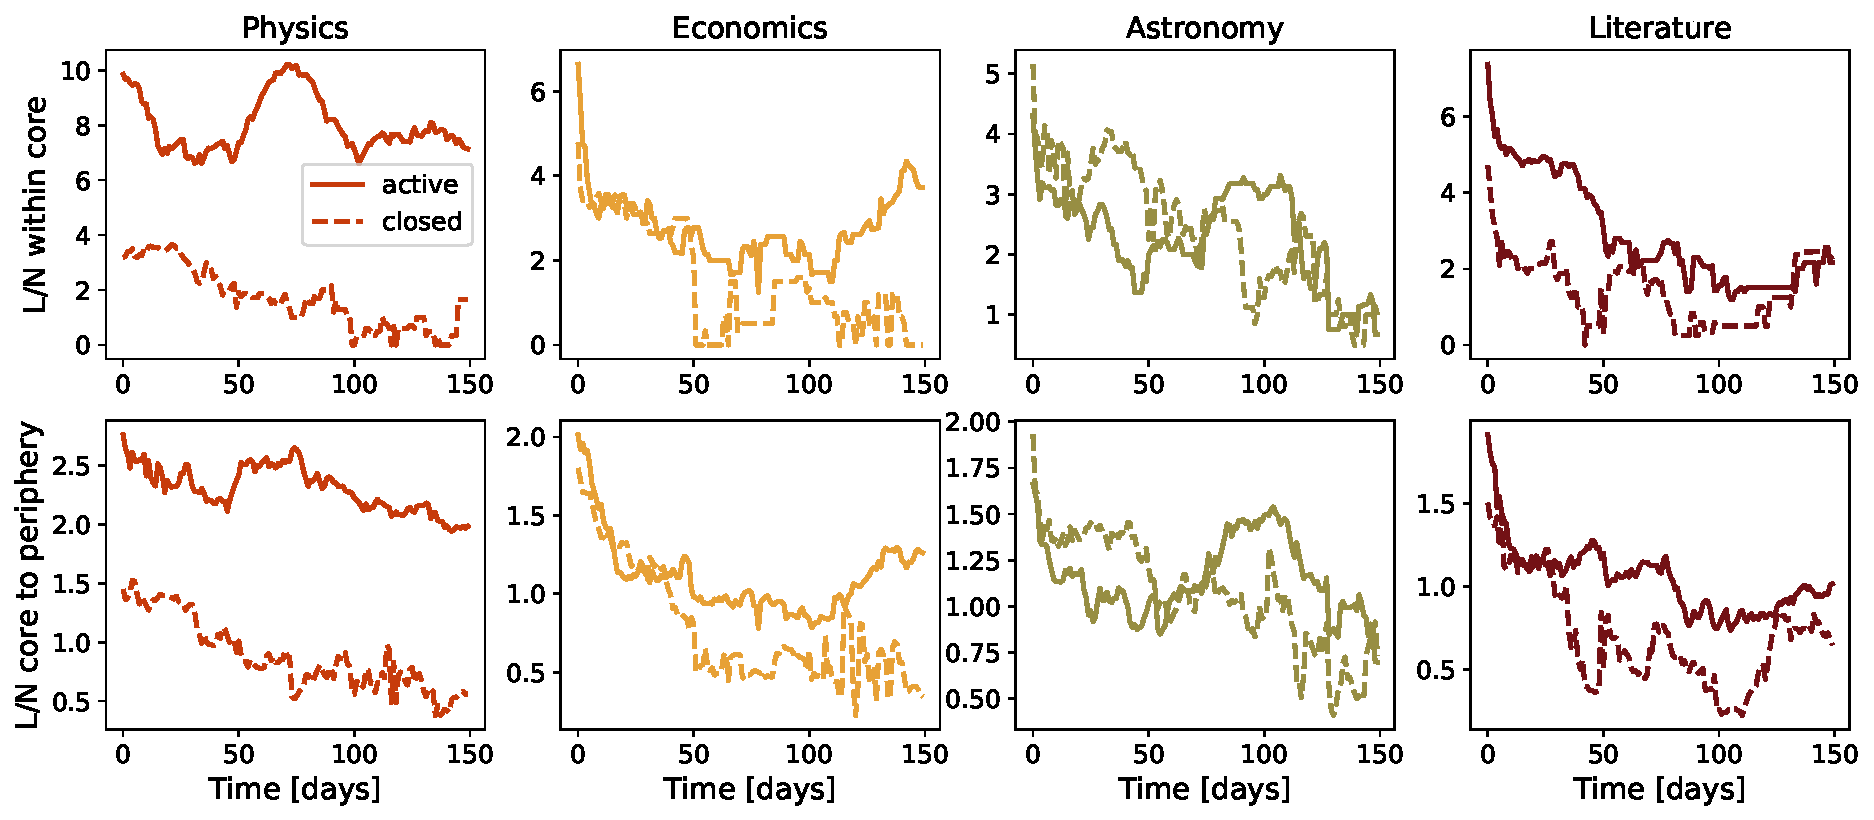
\includegraphics[width=\linewidth]{figures/stackexchange/core_connectivity.pdf}
	\caption{Links per node in core and links per node between core and periphery.}
	\label{fig:links_per_node}
\end{figure}


\subsection{Core-periphery structure of the interaction networks}


In Q-A communities are common two types of users: popular and casual users. Popular users tend to generate the majority of interactions - they are likely to post more questions, also take part in answering questions and tend to engage discussions through comments. For popular users we consider $10 $  of most active users. We analyse interactions between popular and casual users and  among popular users in the  sub-networks of 30 days [t+30). In both cases the number of links per nodes in active sites are larger than in closed communities (figure \ref{fig:pop_cas_users}).

Although this separation of users puts an emphasis on  differences between closed and active sites, it does not guarantee that all popular users are in the top 10 . To solve this dilemma we use the SBM (Stochastic Block Model) algorithm) to detect the core and the periphery of each 30 days sub-network. Such a split of users leads us to similar conclusions as before. (see figure \ref{fig:windows} - 2nd column)

Stochastic models start from random configuration and the algorithm  can converge to different local stable states. For each 30 days sub-network we run 50 iterations of SBM and choose the model parameters $\theta, p$ according to minimum description length. As example we show analysis of inferred sample of  core-periphery structures for 30 days area51 astronomy networks, Figure \ref{fig:sample}. We represent mean minimum description length (MDL) and mean number of nodes in the core with standard deviation. MDL does not change much among inferred core-periphery structures, still difference between obtained configurations is notable in the number of nodes in the core.  To investigate in more details similarity between obtained core-periphery configurations in the sample we calculate several measures between pair-wised partitions such as normalized mutual information, adjusted rand index, F1 measure and Jaccard index. Those measures are larger than 0.5, and in most cases higher than 0.9 indicating stability of the inferred core-periphery structures.
%TODO
%. MDL does not change much among infered core-periphery structure, Fig \ref{fig:sample} while looking into adjusted rand index we can notice that difference exists. Still, ARI between pair-wised compared partitions is large ($ari >0.9$) indicating stability of inferred structures.    



To study the stability of the core across the time we compute Jaccard’s coefficient between core users in [t+30) networks selected at times $t_1$ and $t_2$, (figure \ref{fig:jaccard_hm}). Higher values of the Jaccard index indicate that core users tend to stay in the core. The detected cores experience a lot of change over time and the highest overlap between core users is in the network closer in the time. The average Jaccard index between core users in all sub-networks separated by time interval $|t_1 - t_2|$ with standard deviation confidence interval is presented in figure \ref{fig:jaccard_mean}. Compared to closed sites, active sites show more stability in the core. Even the number of core users obtained in the launched and closed communities are comparable \ref{fig:core_size} (a high difference is found only for physics ), the ratio between total core and periphery reputation is evidently higher in the active than in closed sites, figure \ref{fig:dr_core_per}.  

\begin{figure}[h!]
	\centering
	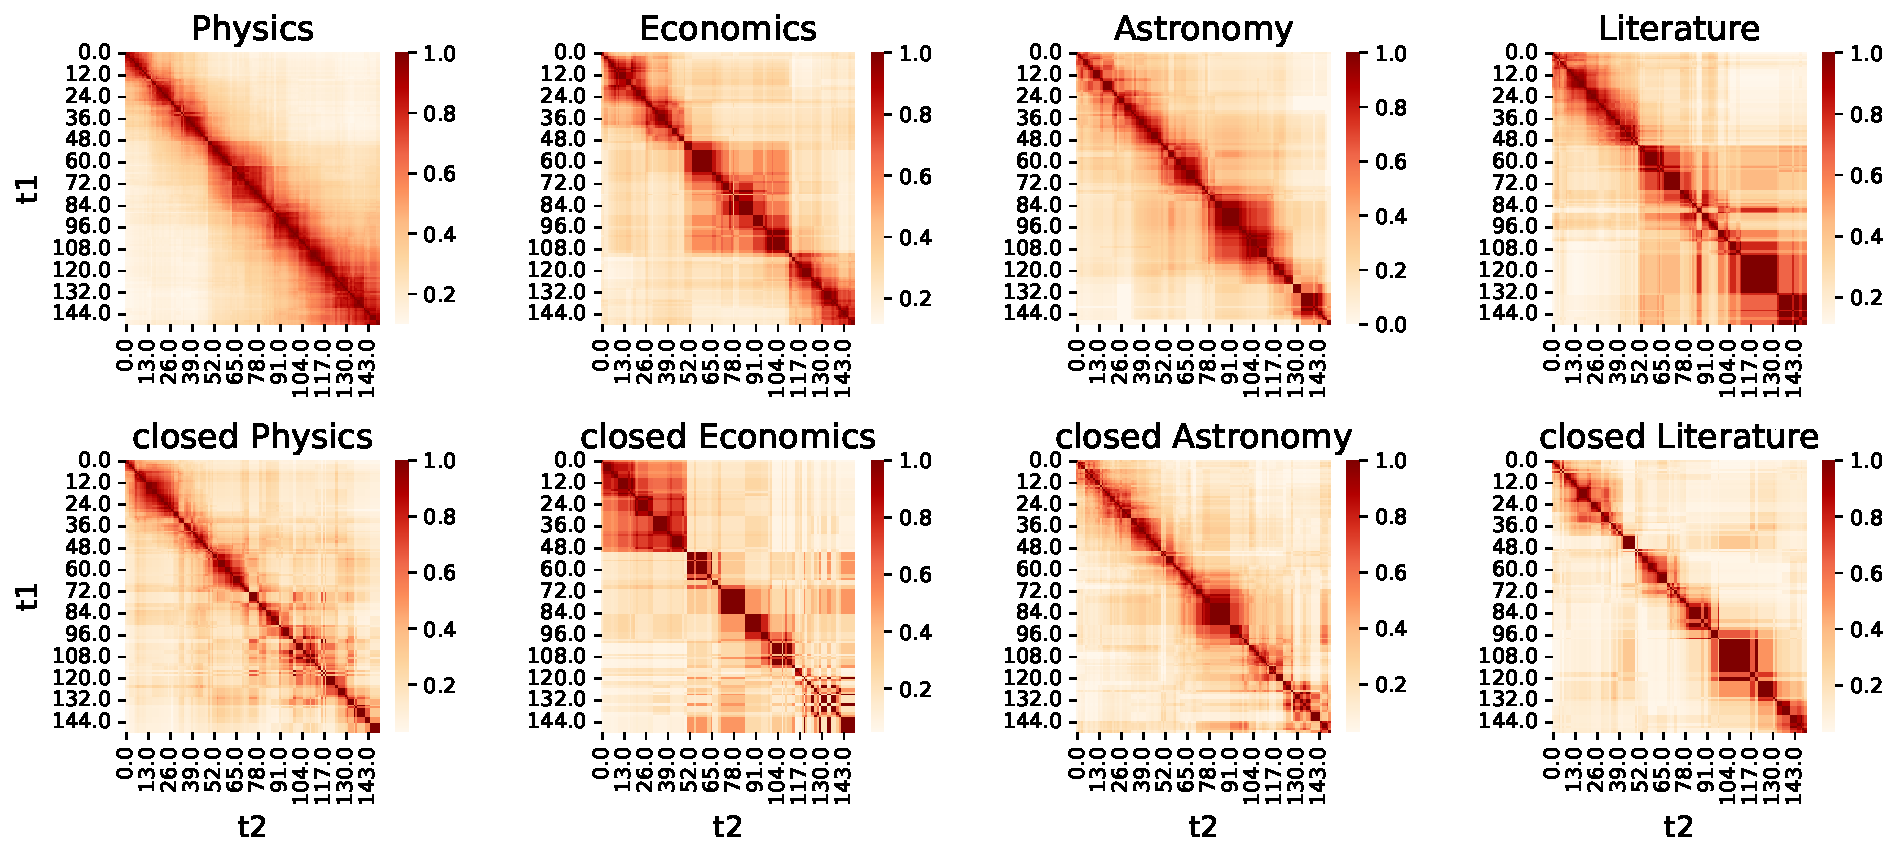
\includegraphics[width=\linewidth]{figures/stackexchange/jaccard_heatmap.pdf}
	\caption{Jaccard index between core users in  sub-networks at time points $t1$ and $t2$}
	\label{fig:jaccard_hm}
\end{figure}

\begin{figure}[h!]
	\centering
	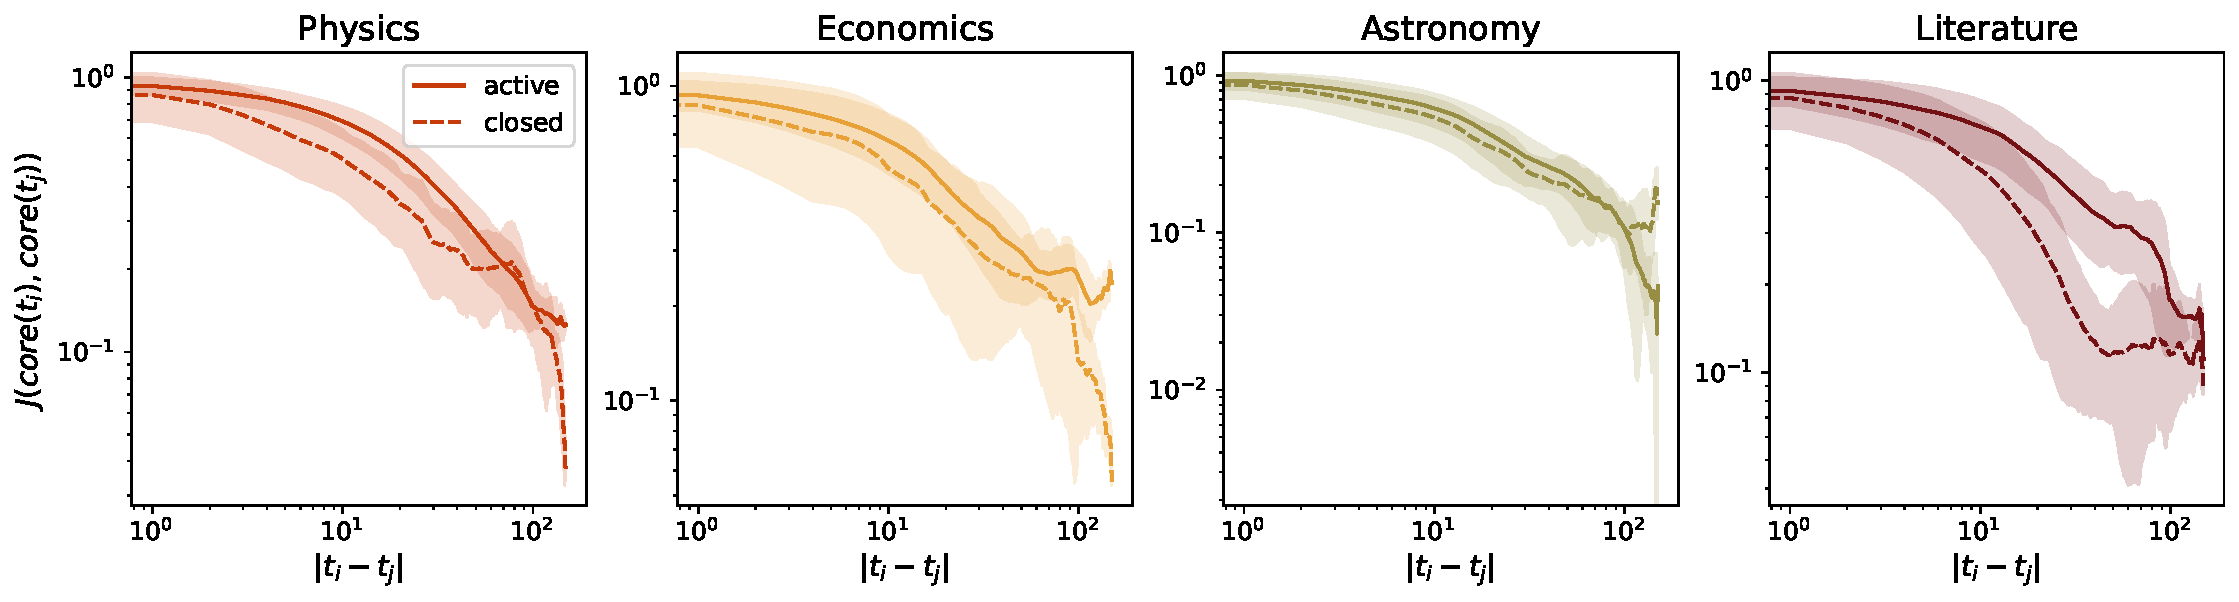
\includegraphics[width=\linewidth]{figures/stackexchange/jaccard.pdf}
	\caption{Jaccard index between core users in 30days sub-networks for all possible pairs of 30 days sub-networks separated by time interval $|t_i - t_j|$}
	\label{fig:jaccard_mean}
\end{figure}

% mozda bi ove dve slike core size i ration between reputations mogli da spojimo (slike A9 i A10), samo da se doda treci red na A9? 

\begin{figure}[h!]
	\centering
	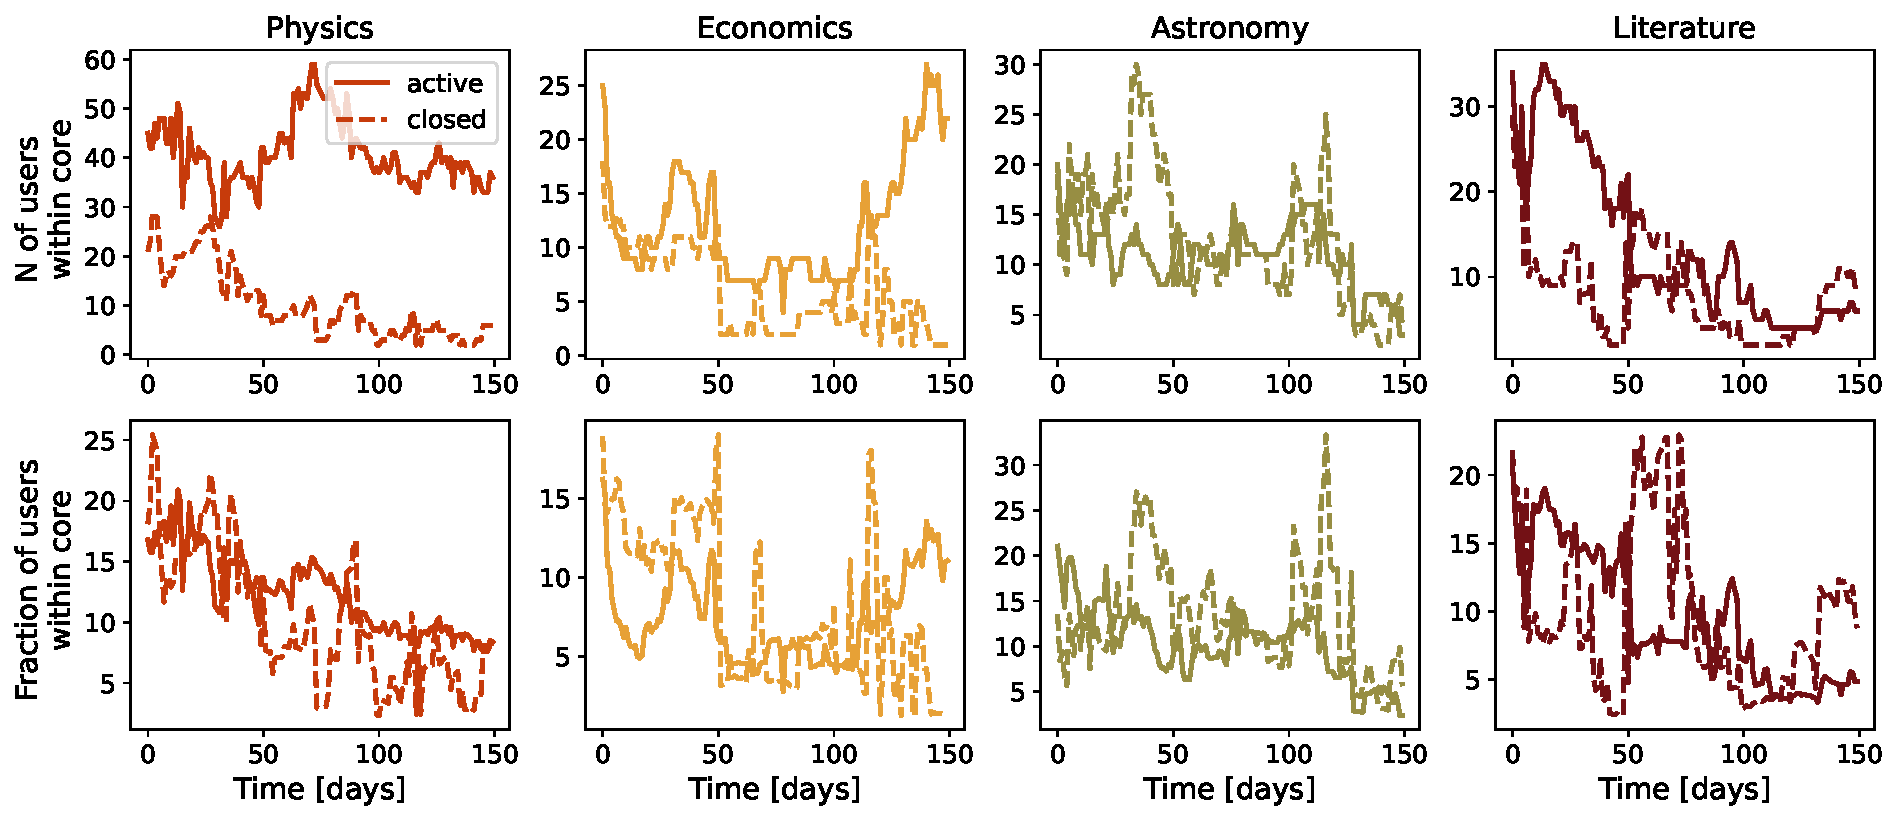
\includegraphics[width=\linewidth]{figures/stackexchange/core_users.pdf}
	\caption{Just for reference size of the core (top) and fraction of users in core (bottom). Solid lines - active sites; dashed lines - closed sites.}
	\label{fig:core_size}
\end{figure}

\begin{figure}[h!]
	\centering
	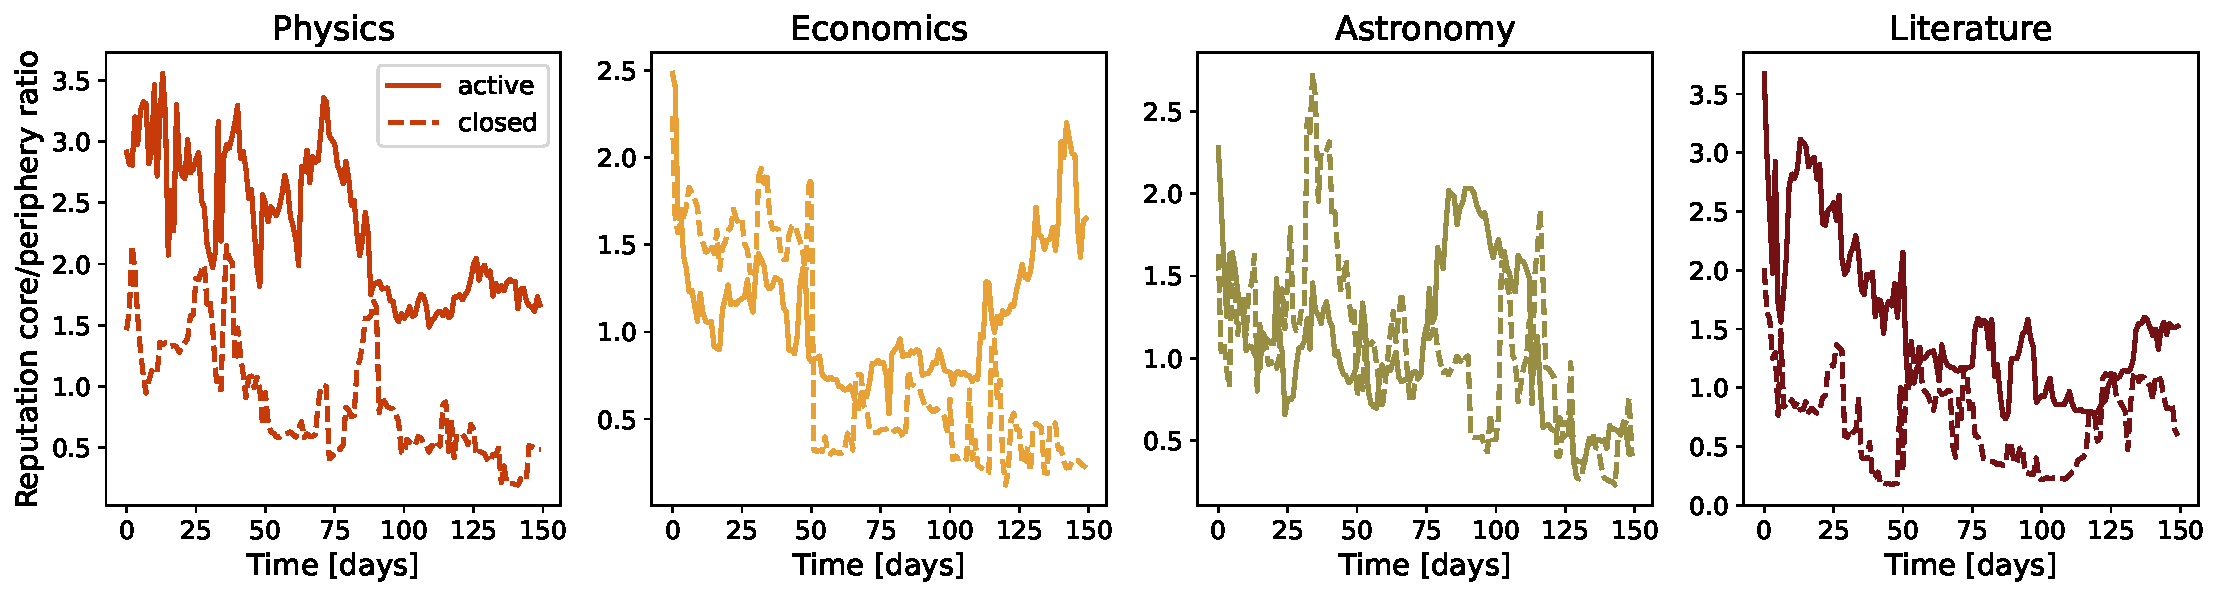
\includegraphics[width=\linewidth]{figures/stackexchange/core_per_ratio_reputation.pdf}
	\caption{Ratio between the total reputation within network core and periphery. Solid lines beta communities, dashed lines area 51 communities.}
	\label{fig:dr_core_per}
\end{figure}

\clearpage
\begin{figure}[h!]
	\centering
	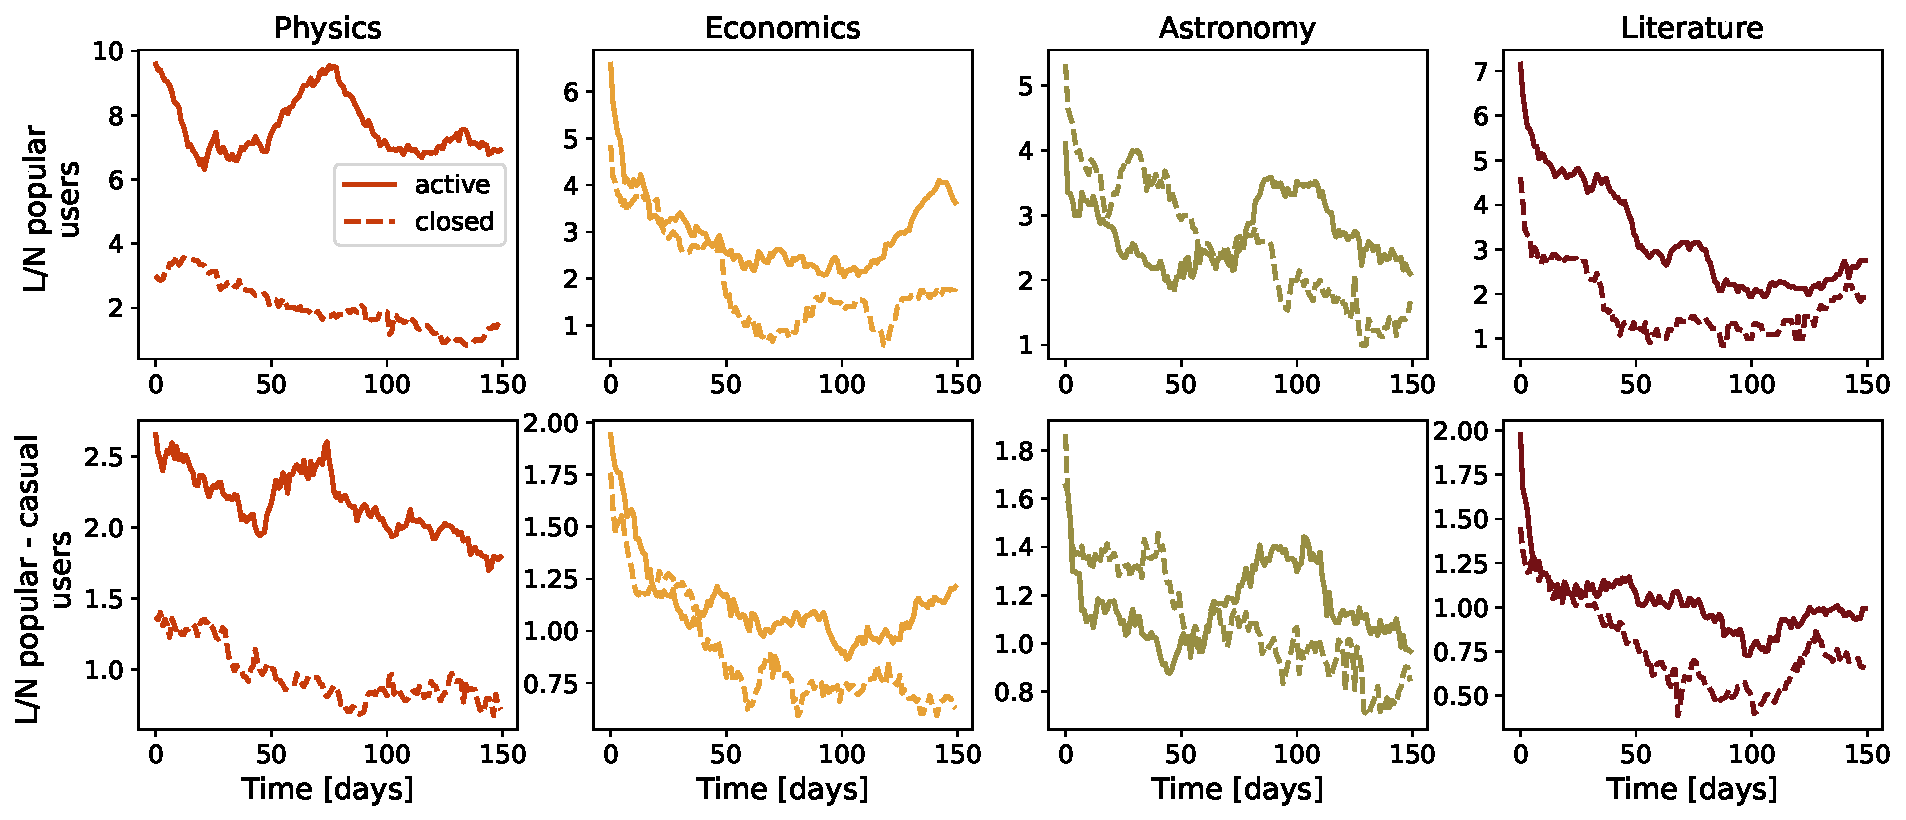
\includegraphics[width=\linewidth]{figures/stackexchange/popular_casual_users.pdf}
	\caption{Links per node among popular users (top 10\% of users) and between popular and casual users (everyone but popular users).
		Reminder: only 3rd and 5th columns should stay and only for reference to previous research, while our point is to this selection via core/periphery decomposition without thresholding.}
	\label{fig:pop_cas_users}
\end{figure}

\section{Dynamical Reputation model}

\subsection{Selection of dynamical reputation model parameters} \label{section:param}
One of the largest drawbacks of DIBRM is the parameter tuning problem. In previous applications of the model \cite{melnikovDynamicInteractionBasedReputation2018,yashkina2020} there was no single best set of parameter values for modeling dynamic reputation in Stack Exchange communities. For example, in \cite{yashkina2020} the best approximation of the official Stack Exchange reputation is obtained with $t_a =2, \beta = 1, \alpha = 1.4$ which means there is no active forgetting factor. In our application of DIBRM to SE communities we opted for a different set of parameter values. Details of parameter search and tuning are presented in SI.

For basic reputation contribution of a single interaction we selected $I_{bn} = 1$ and at the same time this is the threshold value of an active user. This value is intuitive as every interaction has initial contribution of +1 to user's reputation, although the previous works have used values of +2 and +4. Following the previous work and after examining the median/average time between subsequent interactions of the same user, we selected $t_a = 1$, which also means that reputation in our model will be updated every day during the time-window of the analysis, regardless of whether the user is active or not. To emphasize the bursts of activity and frequent recent interactions, cumulative factor has a larger value $\alpha = 2$. Finally, the most delicate parameter is the forgetting factor, which at the same time determines the weight of past interactions and the reputational punishment due to user inactivity. Here we need to select the value of parameter $\beta$ so we include the forgetting due to inactivity but not to penalize is too much. In Fig. A1 we show how different values of parameter $\beta$ influence the time needed for user's reputation to fall on value $I_{n}=1$ due to user's inactivity and value of dynamical reputation in the moment of the last activity. The higher the value of parameter $\beta$ and initial dynamical reputation of users, the longer time it takes for user's reputation to fall on baseline value. For parameter $\beta=0.9$ and $I_{n}=5$, user's reputation falls on value $I_{n}=1$ after less than 20 days, while this time is doubled for $\beta=0.96$. We see, that for higher values of parameter $\beta$ the time needed for $I_{n}$ to fall on value $1$ becomes longer, and that the the initial value of reputation becomes less important. 

Figure A2 in SI shows the difference between the number of users that had at least one activity in the window of 30 days and number of users with reputation higher than $1$ during the same period for different values of parameter $\beta$. The minimal difference between these two variables is observed for the values of $\beta$ between $0.94$ and $0.96$ for both live and closed communities. Since we want to compare communities, we select $\beta = 0.96$ after verifying that this level of reputational decay does not reduce the number of active users (based on their dynamic reputation) below the actual number of users who have been active (interacted with the community) in the time window of 30 days. 

To summarize, our model of dynamical reputation has three parameters: 1) basic reputation contribution $I_{bn}=1$; 2) cumulative factor $\alpha=2$; 3) forgetting factor $\beta=0.96$. The selected values of parameters are used for measuring dynamical reputation of user in all four pair SE communities. Given these values of parameters, the minimal reputation achieved by the user immediately after they have made an interaction in the SE community is $1$. This reputation will decay below $1$ if the user does not perform another interaction within the one-day time window. For any user in a community, when their reputation drops below $1$, we consider this user inactive which means that the user at that time is not "visible" in the community and their past contributions at that time are unlikely to impact other users. The number of active users and mean user reputation for different Stack Exchange communities are shown in Fig. \ref{fig:dr6panel}.

\subsection{Dynamic reputation - $\beta$ parameter}

Our implementation of dynamic reputation model was based on $\beta = 0.96$. There are several reasons for selecting this value.

In Dynamic reputation model, the $\beta$ parameter controls the strength of the forgetting fator of the model.  The value of this parameter should reflect the core feature of the reputational systems and make reputation easier to loose. Due to user's inactivity, any level of reputation will eventually decay to below 1. Dependence of time needed for reputation to drop below this level and the $\beta$ parameter, as well as reputation before inactivity is shown on Figure~\ref{fig:betadelta}. Here $I_n$ is equal to the raw number of interactions in the community without forgetting or cumulative factor at work.

\begin{figure}[h!]
	\centering
	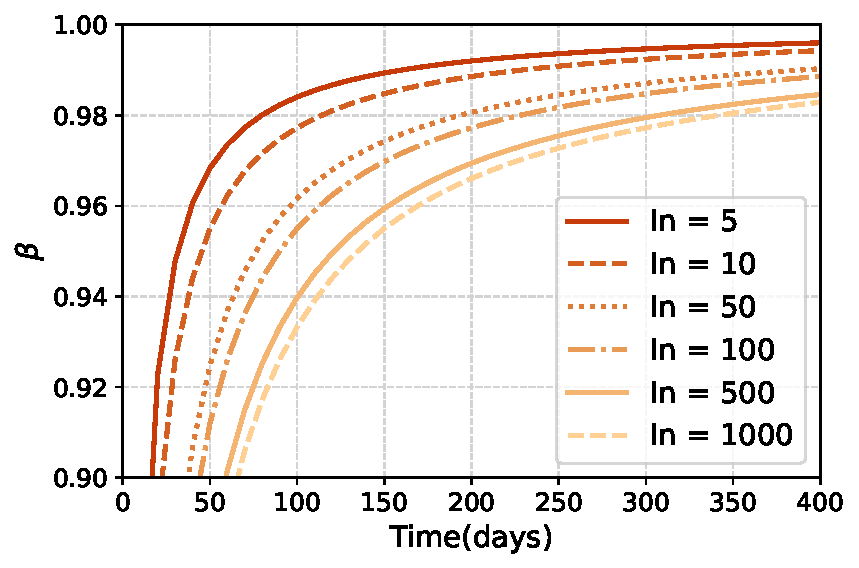
\includegraphics[width=0.5\linewidth]{figures/stackexchange/reputation_decay.pdf}
	% REMOVE 'SLOWER' FROM THE PLOT TITLE > zamenjeno i formulu sam prebacila u caption
	\caption{Dependence of parameter $\beta$ and number of days $\Delta$ needed for reputation $I_n$ to drop to $I_{n_0} = 1$. Dependence of parameter $\beta$ and number of days when reputation due inactivity decreases from $I_n$ to $I_0$ is given as  $\beta = (\frac{I_{n0}}{I_{n}})^{(1/\Delta)}$ }
	\label{fig:betadelta}
\end{figure}

\begin{figure}[h!]
	\centering
	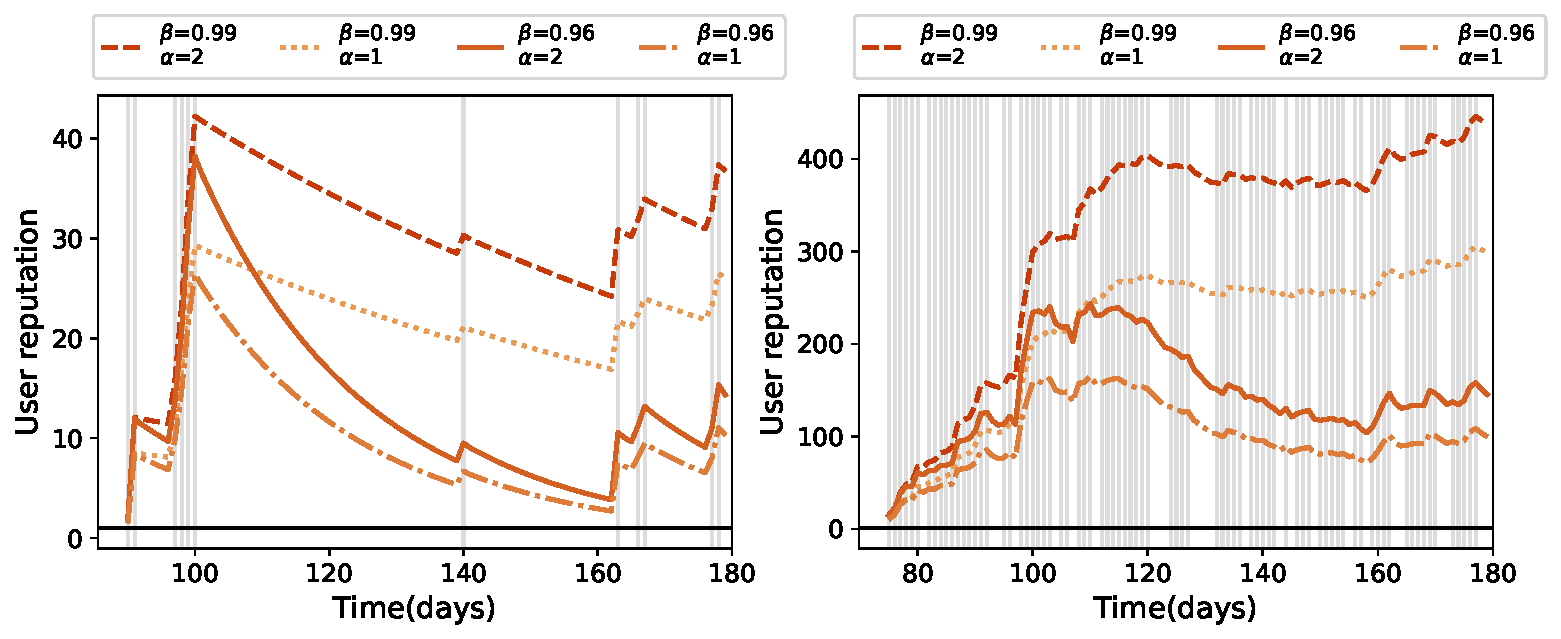
\includegraphics[width=\linewidth]{figures/stackexchange/single_user_reputation.pdf}
	% REMOVE 'SLOWER' FROM THE PLOT TITLE > zamenjeno i formulu sam prebacila u caption
	\caption{Single users reputations }
	\label{fig:singleuser}
\end{figure}

For $\beta$ values below 0.96, the decay is fast and within two to four months of inactivity even high values of reputation are reduced below the threshold. On the other hand, with $\beta$ values the decay proces is more differentiated and high reputation becomes harder to loose, surviving up to a year of inactivity. For $\beta$ equal to 0.96, it takes a month for reputation based on 5 interactions to decay and around five months for high reputation based on 500 or 1000 interactions to decay below the threshold.

\textbf{30 days sliding window} We compared the number of users with estimated reputation higher than 1 for different parameters $\beta$ and concluded that $\beta$ close to $0.96$ approximates the number of users with recorded interactions in a given 30 days sliding window. For each pair of communities we calculated number of users with at least one interactions in every 30 days sliding window and then we estimated several times series expressing the number of users with reputation higher than 1 for fixed $\beta$. Then we calculated the root mean square error (RMSE) between those time series for the first 200 days. Values of RMSE are shown on Figure~\ref{fig:rmse}. For each community, we can find parameter $\beta$ that minimizes RMSE. Although $\beta$ does not have a unique value across communities, it varies between 0.95 and 0.96. 
%We should notice that taking different time period, for example, the first 90 days, we can get different optimal values of betta, but they'll probably take values between 0.95 and 0.96 (I can test it). 


\begin{figure}[h!]
	\centering
	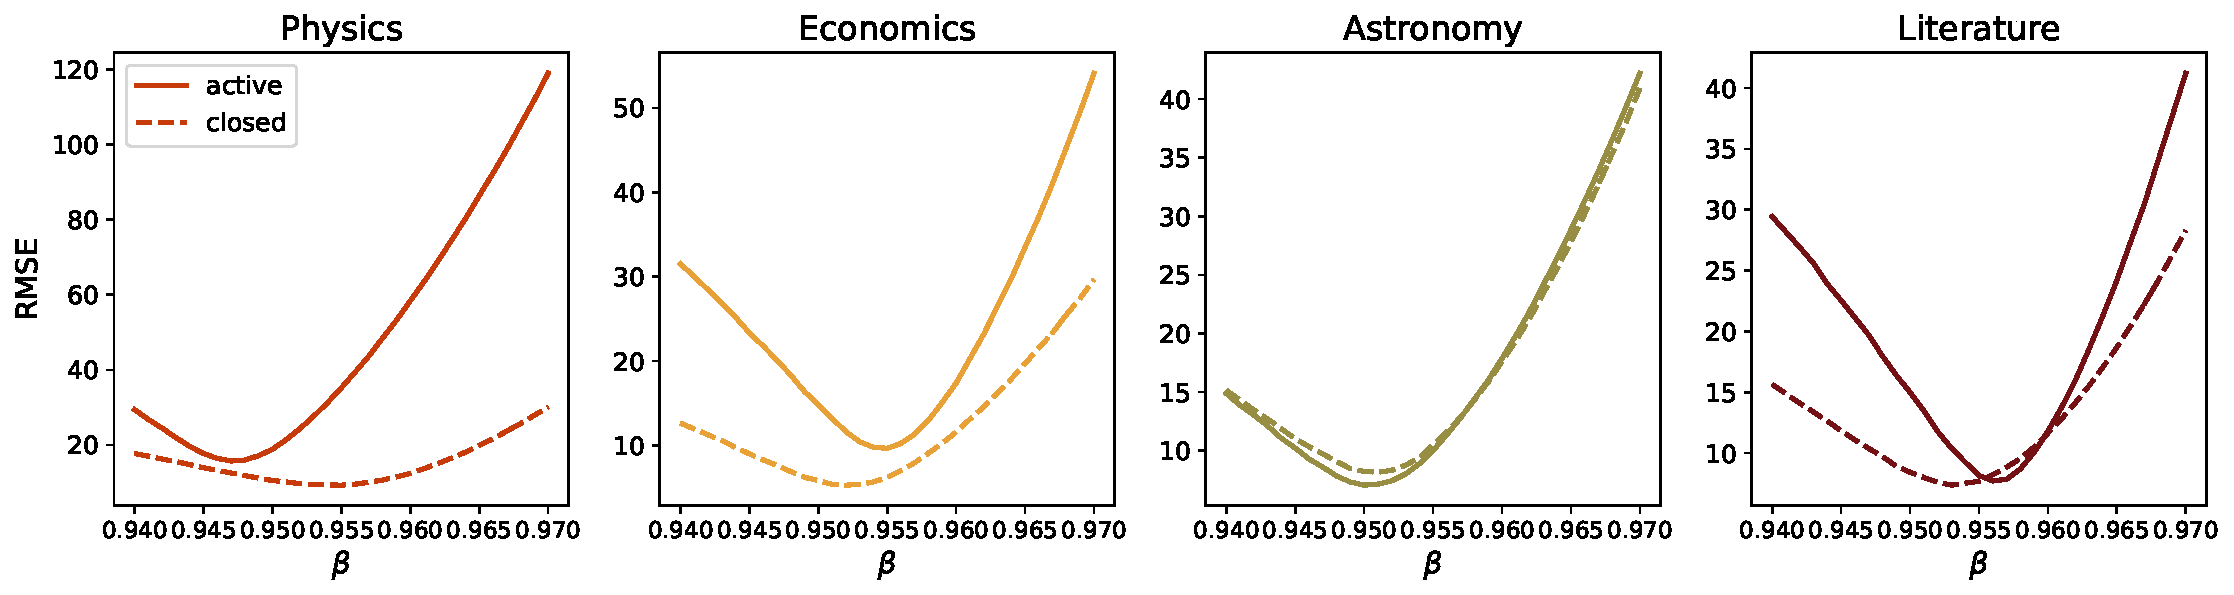
\includegraphics[width=\linewidth]{figures/stackexchange/rmse.pdf}
	\caption{RMSE between number of active users in sliding window of 30 days and number of users with reputation $>1$ for  $0.94< \beta <0.97$ with step $0.001$. }
	\label{fig:rmse}
\end{figure}

Figure \ref{fig:nusers} shows comparison between number of users in 30 days sliding window, number of users for these optimal values $\beta = 0.954$ and $\beta =0.96$. For $\beta = 0.96$ we observe that in most communities estimated number of active users consistently slightly higher than the actual number of users which have made at least one interaction in that sliding window. This means that dynamic reputation model in some cases overestimates the reputation of the user, but far more important is that it never understimates the real number of active users. Since we base our calculations of total and average reputation within the community only on users whose reputation is higher than the threshold this is important as no active users are disregarded by the model due to the value of the decay parameter.

\begin{figure}[h!]
	\centering
	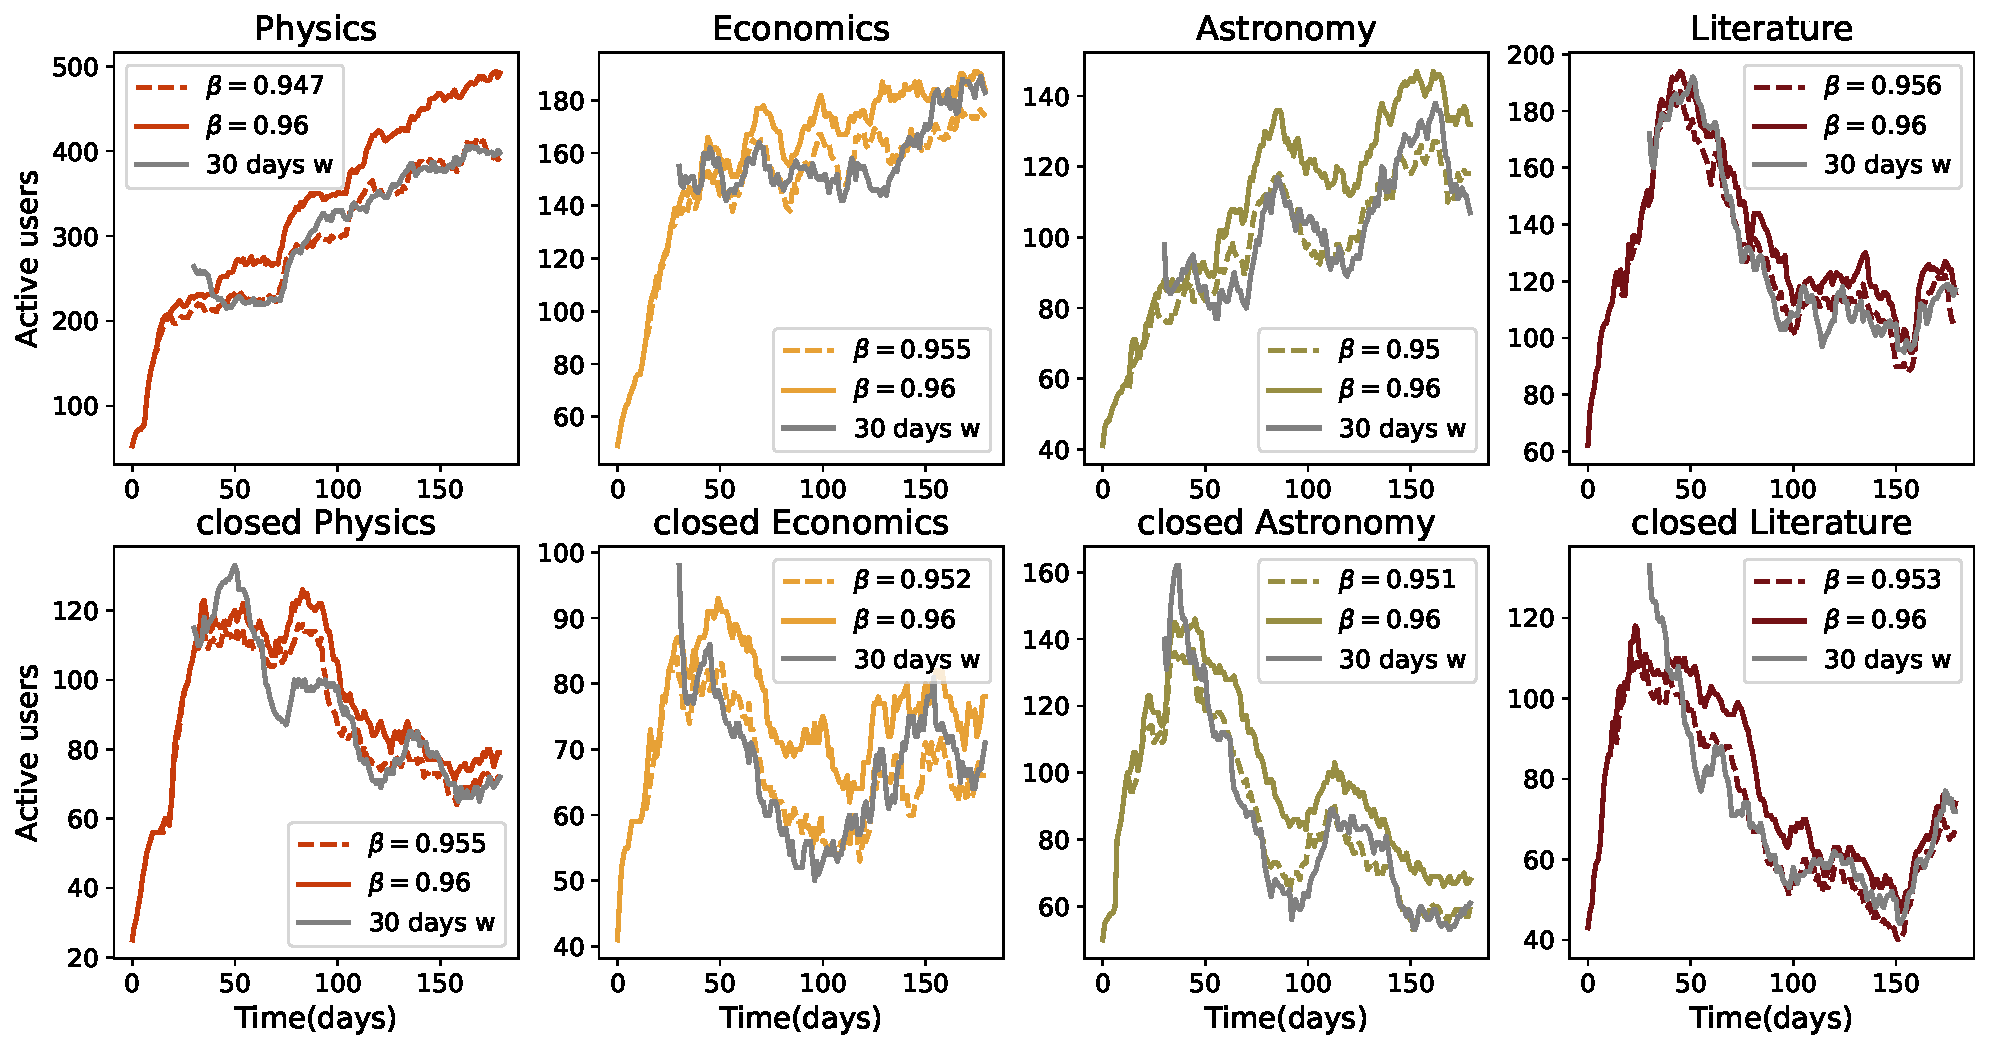
\includegraphics[width=\linewidth]{figures/stackexchange/active_users.pdf}
	\caption{Number of active users in a sliding window of 30 days and number of users with dynamic reputation higher than 1 for $\beta=0.954$ and $\beta=0.96 $ which provide the best fit to the number of users in 30 days sub-networks for each community}
	\label{fig:nusers}
\end{figure}

Finally, it's imporant that our dynamic reptuation captures the trend of long-term user activity. In Figure~\ref{fig:active-users} solid lines show the time series of estimated dynamic reputation for $\beta = 0.96$ while dashed lines show the number of users who were active in a given sliding window and continued to be active in the next one. Although the total estimated number of active users is expectedly higher, two time series follow similar trends in different communities.

\begin{figure}[h!]
	\centering
	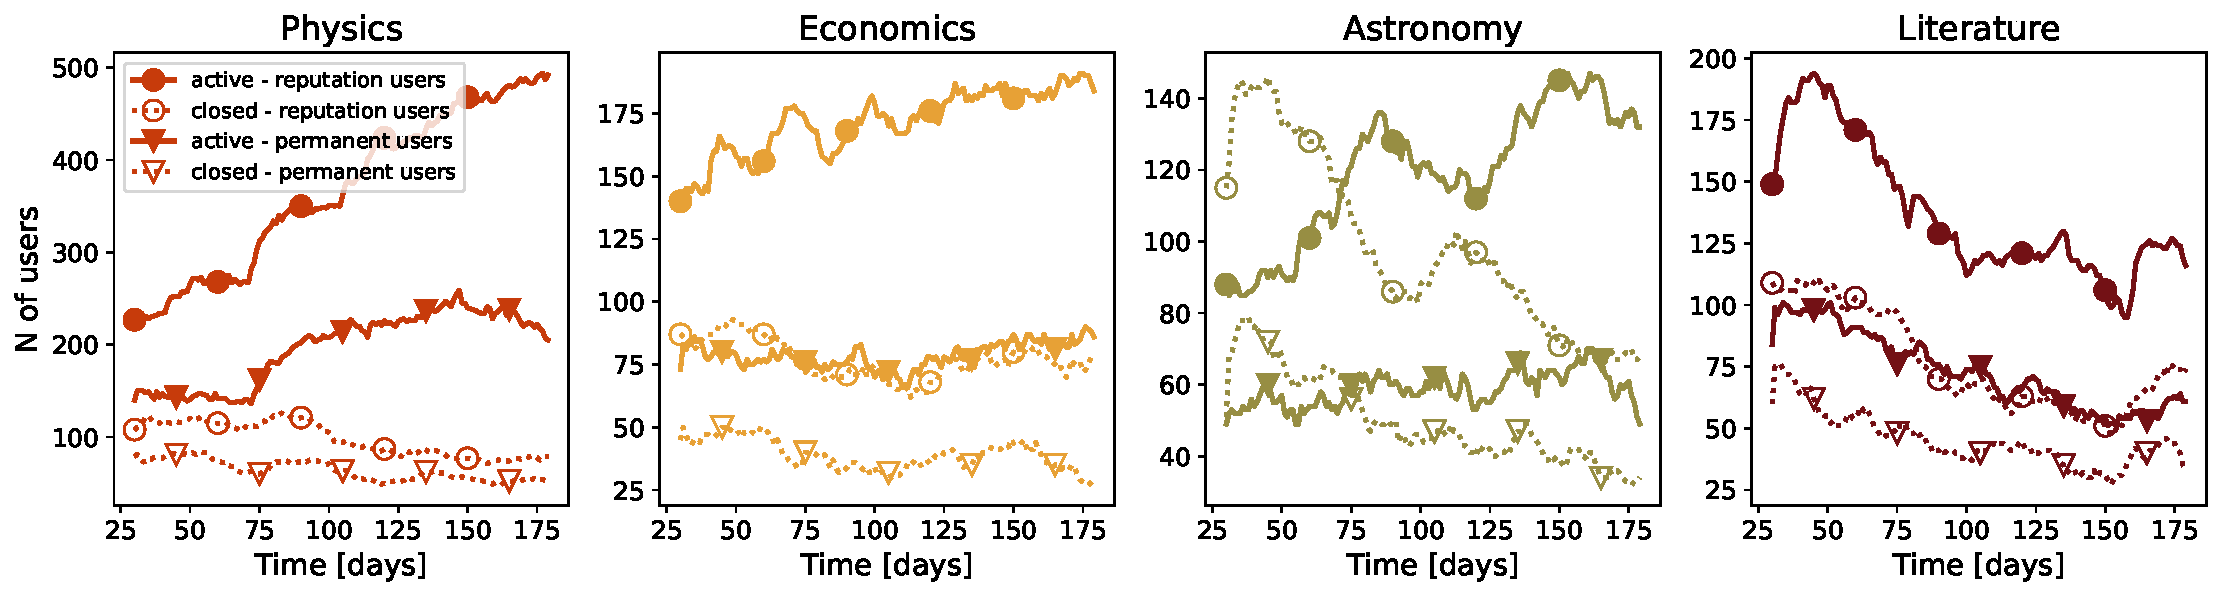
\includegraphics[width=1\linewidth]{figures/stackexchange/permanent_users.pdf}
	\caption{Solid lines represent number of users with dynamic reputation higher than 1 for $\beta=0.96$ while dashed lines are number of users within 30 days sliding window who were active and remained to be active. Blue lines are beta, while red lines are area51 communities.}
	\label{fig:active-users}
\end{figure}
\clearpage




\subsection{Dynamic reputation of users within the network of interactions}

\begin{figure}
	%%% 6 panels
	%%% columns: Total rep., Mean rep., Number of Active Users
	%%% rows 1: Physics. Theo. Physics, Econ. Beta, Econ. A51
	%%% rows 2: Astro Beta, Astro A51, Lit Beta, Lit A51
	\centering
	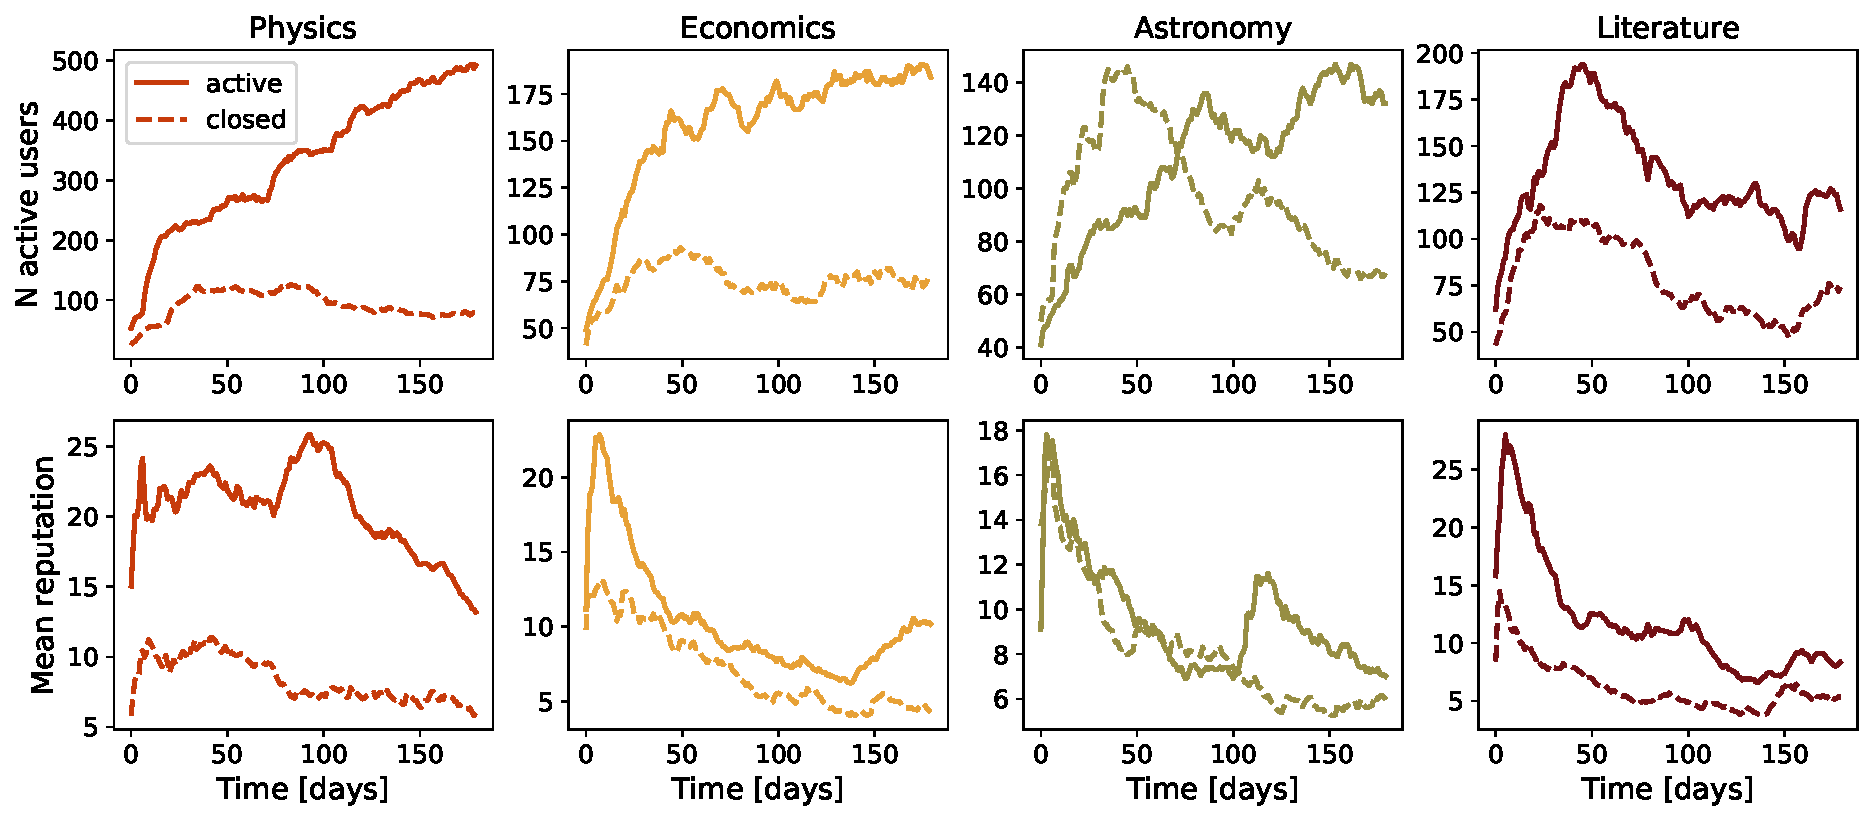
\includegraphics[width=\linewidth]{figures/stackexchange/reputation.pdf}
	\caption{Dynamic Reputation on the four pairs of Stack Exchange websites: Astronomy, Literature, Economics,  Physics and Theoretical Physics.}
	\label{fig:dr6panel}
\end{figure}

\begin{figure}
	\centering
	%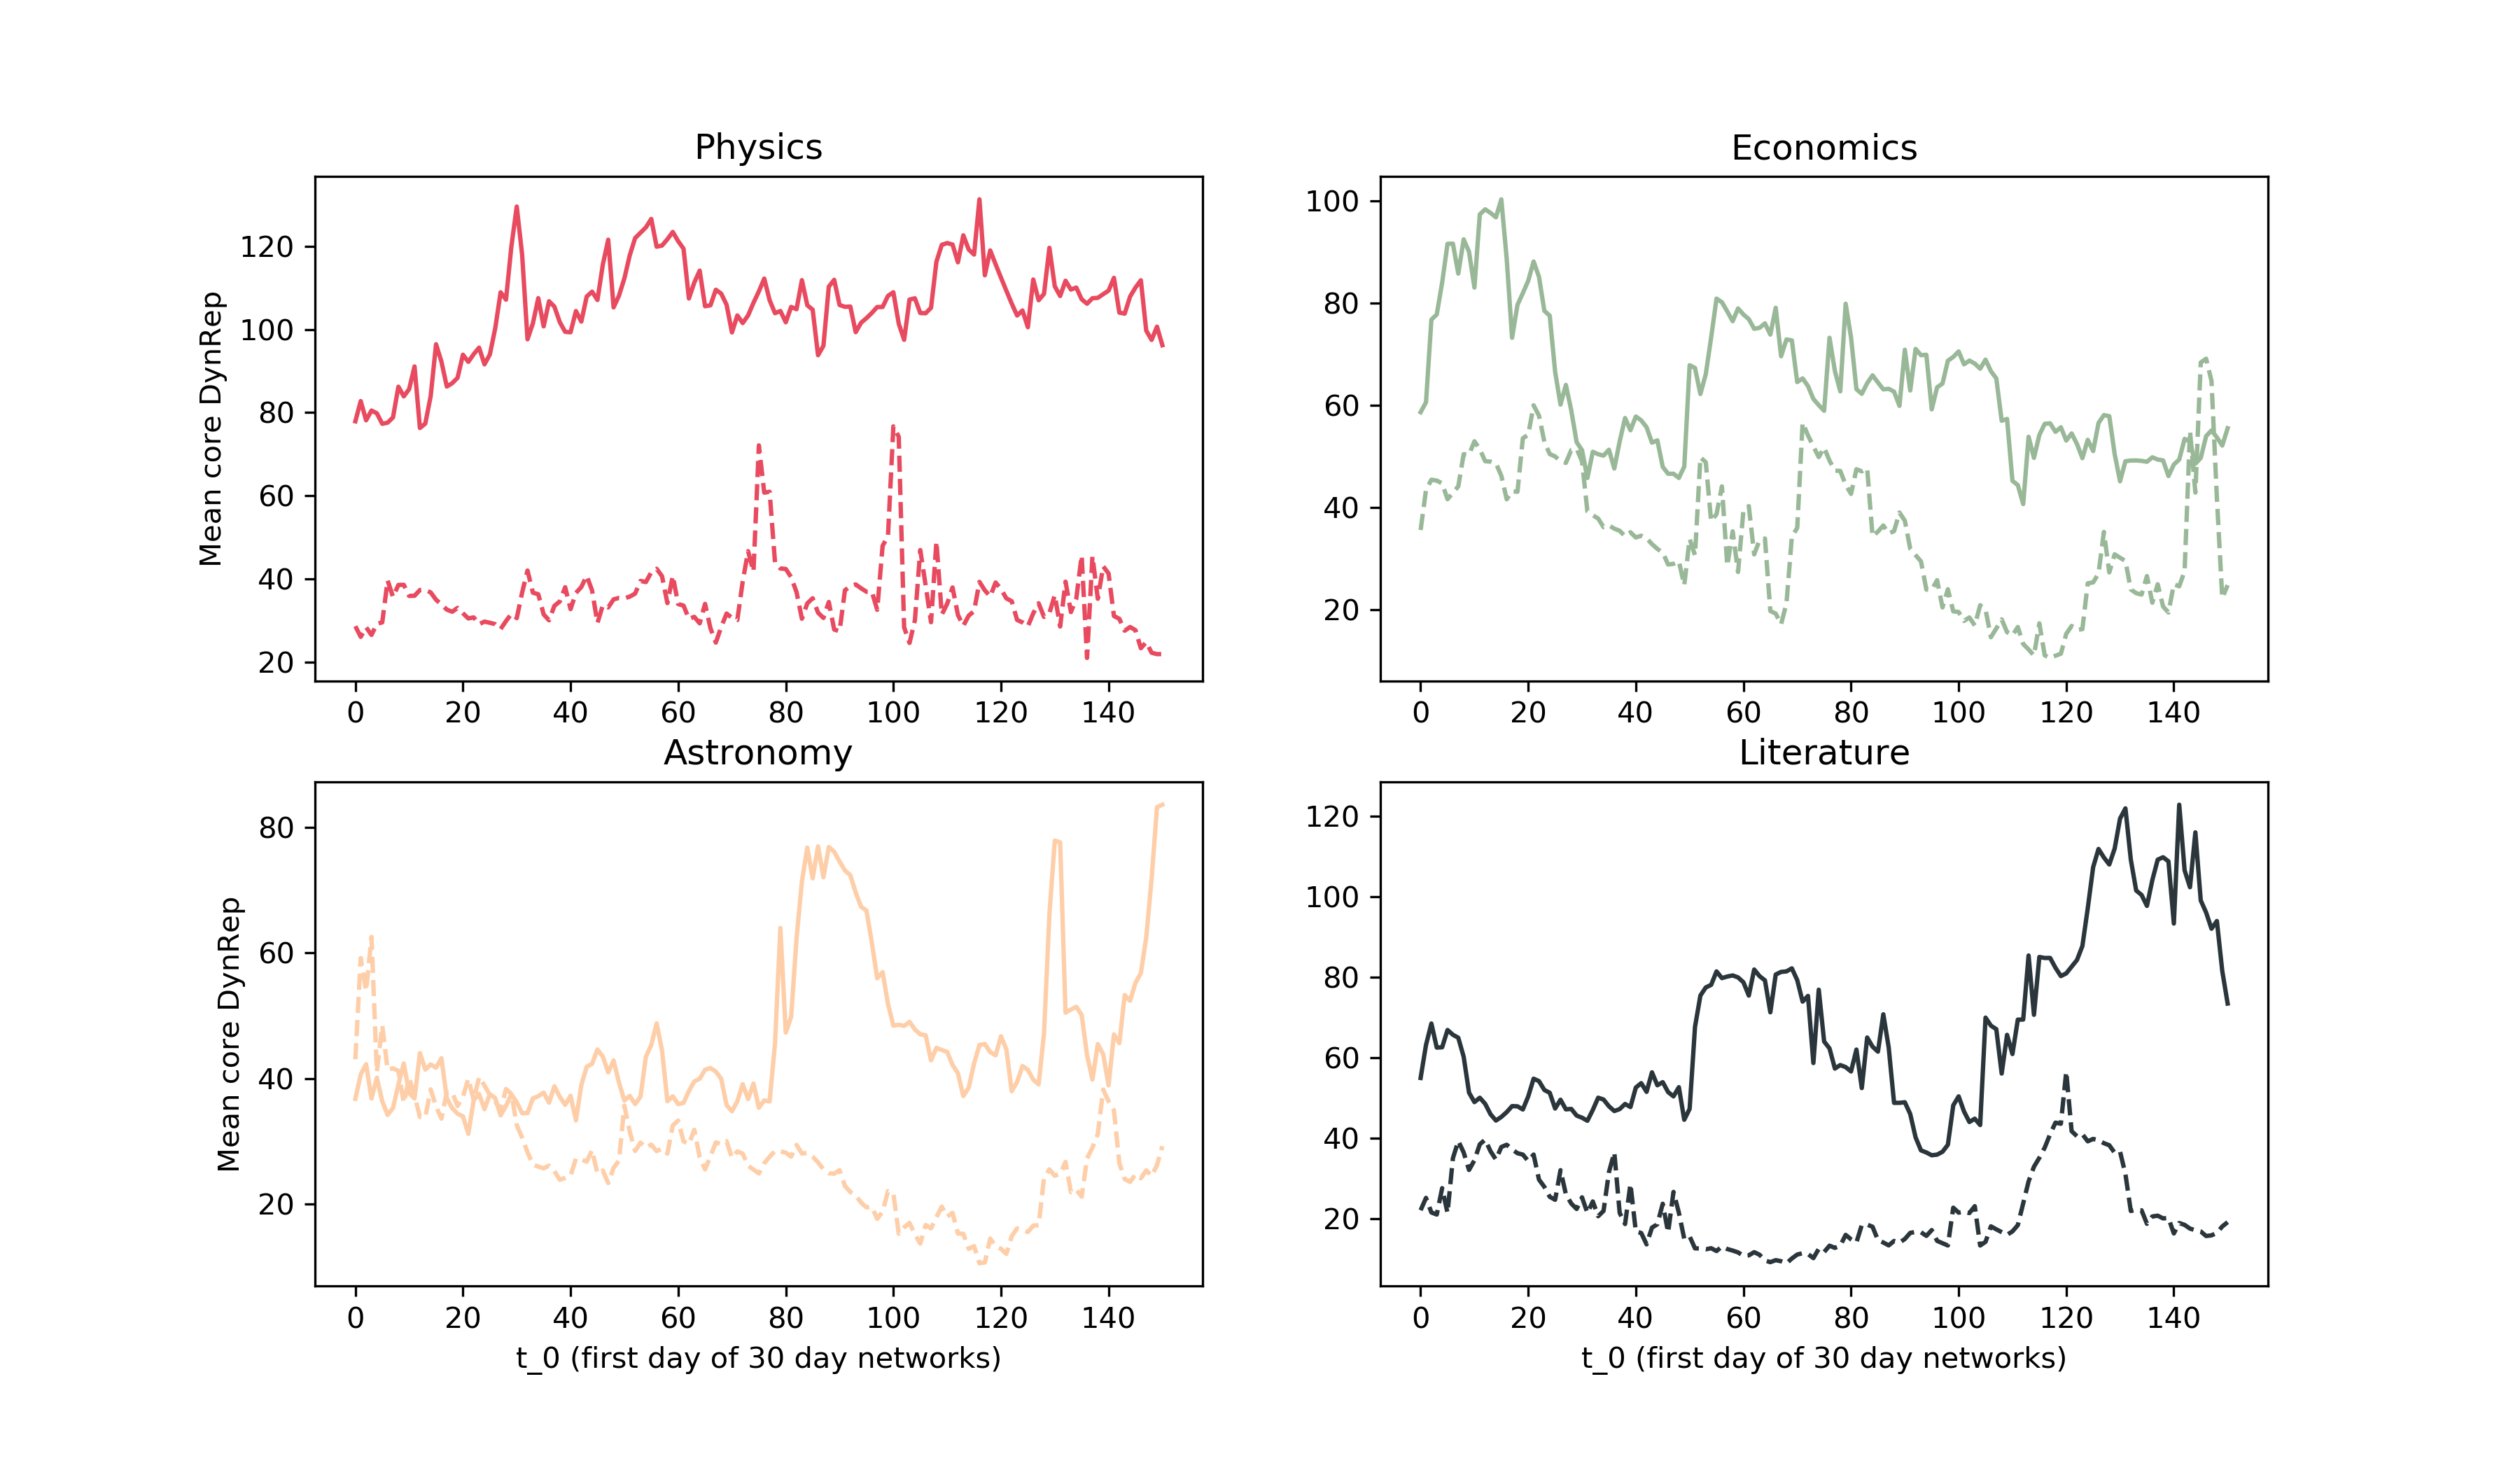
\includegraphics[width=\linewidth]{figures/Mean_core_dyn_rep.png}
	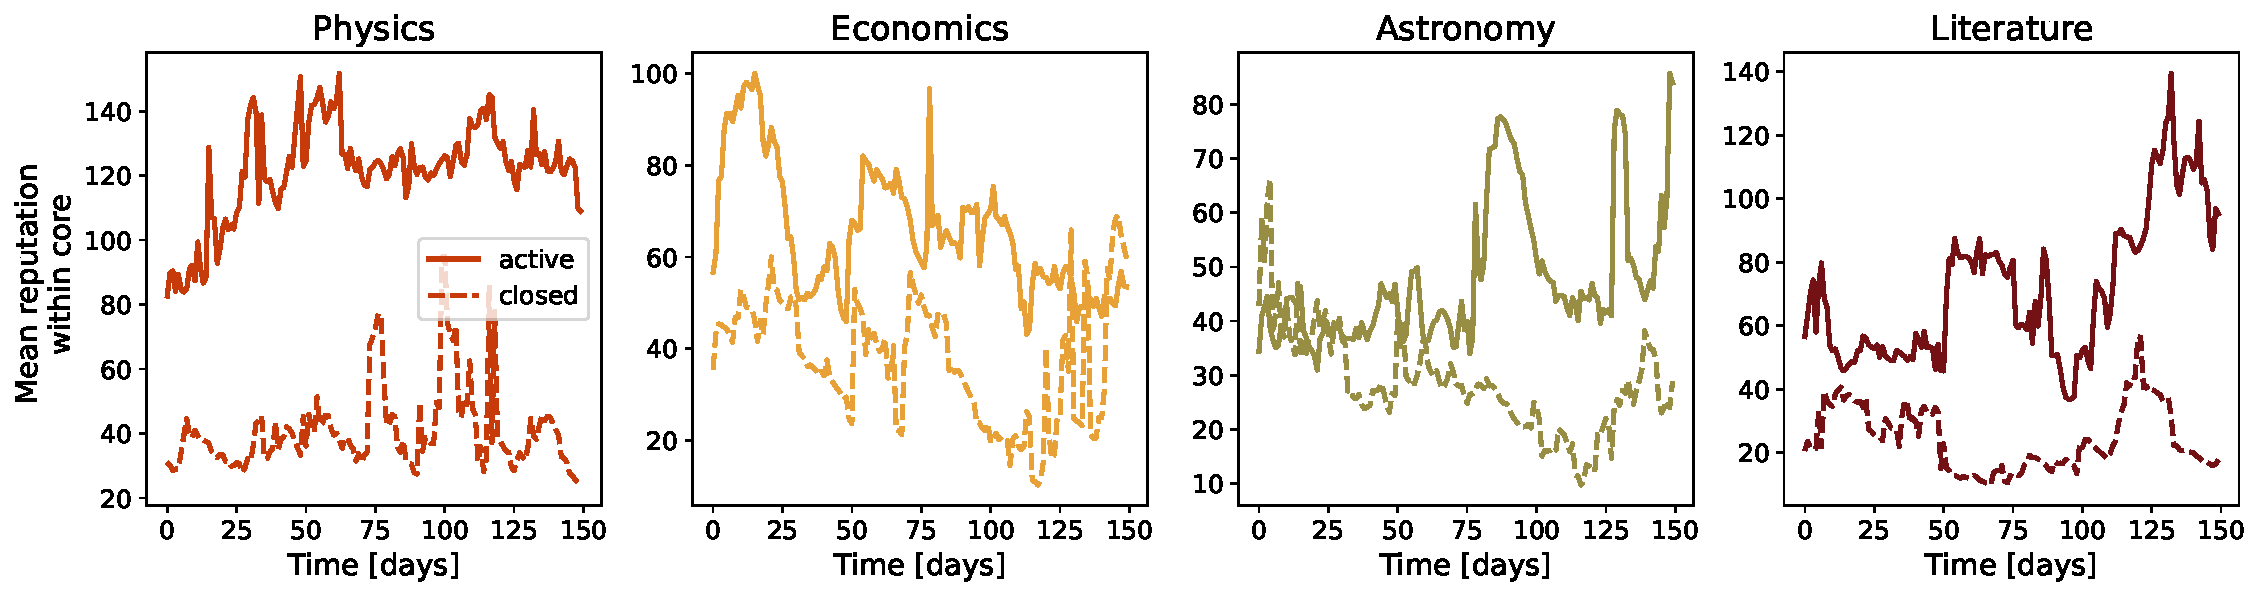
\includegraphics[width=\linewidth]{figures/stackexchange/core_reputation.pdf}
	\caption{Dynamical reputation within core.}
	\label{fig:dr_core}
\end{figure}

Examined network properties suggest that there are structural differences between active and closed communities. Active communities have higher and more stable local cohesiveness compared to their closed counterparts. The overlap of the set of nodes in the core for active communities shows a significant overlap even for distant subnetworks, meaning that the membership of the core in active communities is more stable.

To further explore the differences between active and closed communities, we focus on dynamical reputation which is our proxy for collective trust in these communities. We investigate whether and how core-periphery structure is related to collective trust in the network. Figure \ref{fig:dr_core} shows the mean dynamical reputation in the core of active and closed communities and its evolution during the observation period. There are clear differences between active and closed communities when it comes to dynamical reputation. The mean dynamical reputation of core users is always higher in active communities than in closed. As expected, the largest difference is observed between Physics and Theoretical Physics community. The difference between active communities which are still in the beta phase and their closed counterparts is not as prominent, however, the active communities have higher mean dynamical reputation especially in the later phase of community life. The only difference in the pattern is observed for astronomy communities at the early phase of their life, when closed community has a higher value of dynamical reputation than active community. This is in line with similar patterns in the evolution of mean clustering and core-periphery structure. 

By definition, the core consists of very active individuals and thus we expect higher total dynamical reputation of users in the core in comparison to the the total reputation of users belonging to subnetworks periphery. Figure A12 shows the ratio between the total reputation of core and periphery for closed and active communities and its evolution. The ratio between total reputation of core and periphery in Physics is always higher than in the Theoretical physics community. Similar pattern can be observed for literature communities, although the difference is not as clear as in the case of physics. Ratio of total dynamical reputation between core and periphery is higher for closed community than active one on the economics topic in the early days of community life. However, in the later stage of their lives this ratio becomes higher for active communities. Communities around astronomy topic deviate from this pattern, which once again shows the specificity of these communities. 

To complete the description of the evolution of dynamic reputation active and closed communities, we examine the evolution of Gini index of dynamical reputation in the whole network which is shown in Fig. A5 in Supplementary Information. The Gini index is always higher for active communities than for closed ones, especially for later times in observation period. Only pattern of Astronomy communities deviates from the pattern observed for other three pairs during the early days. These results indicate that the dynamical reputation is distributed in the population more unequally in the active than in closed communities. The evolution of assortativity coefficient that measures correlations between dynamical reputation of connected users in the subnetworks, shown in Fig. A6, shows that networks are disassortative for the largest part of the observation period. These results suggest that users with high dynamical reputation have tendency to connect with users with low value of dynamical reputation. 


In Figure~\ref{fig:dyn_rep_coreper} we show mean user reputation in core and in periphery over time (30 day sliding windows as before). We see that the mean user reputation in core is greater in the currently active sites (solid lines, top panels) than in their closed pairs (dashed lines). In the bottom panels, we see that the mean reputation on the network periphery has substantially lower values, and the difference between active and closed sites is less pronounced. 

For reference in Fig~\ref{fig:core_size} we show core sizes in all sites. We show these in absolute numbers (total number of nodes) and as a fraction of network size through time.






\textbf{Gini coefficient}
Besides the number of active users (who at given moment of observation have reputation higher than the threshold) and the population mean value of dynamical reptuation, we have investigated in more details the distribution of dynamical reputation within discussed communities. We have observed that the distributions are often skewed which prompted us to compare the communities in terms of their Gini coefficient. The gini coefficient is a simple measure that shows us the degree of reputation inequality within the community. We calculate the value based on the dynamic reputation values of users at every time step (day) and report he values in Fig.~\ref{fig:dynrep-gini}. We see that all communities (both still active and closed ones) have gini coeffiecinet values higher than $0.5$ throughout first six month period. Interestingly, except in the case of Astronomy, currently active communities had higher reputation inequality every day during first six month period. As in many other measures, in the case of astronomy, closed community started as more unequal one (signalled by higher gini coef values), but after around two months the situation changed. 
\begin{figure}[h!]
	\centering
	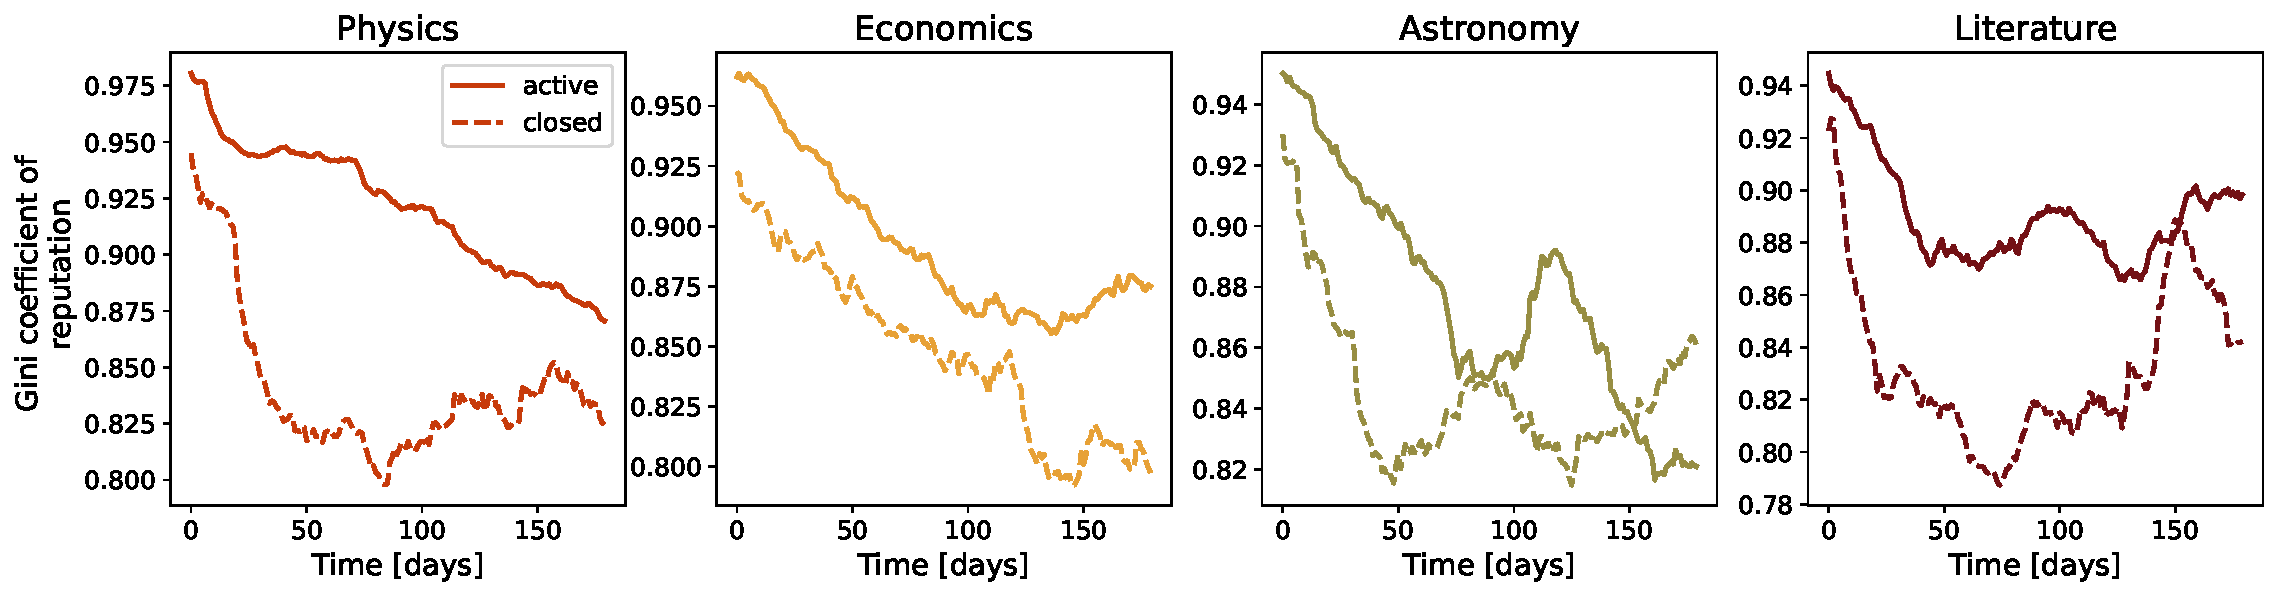
\includegraphics[width=1\linewidth]{figures/stackexchange/gini.pdf}
	\caption{Gini index of dynamic reputation within population}
	\label{fig:dynrep-gini}
\end{figure}

\subsection{Dynamic reputation in the network of interactions}
In the few figures below, we investigate whether users' dynamic reputation is related with users' position within the network.

\textbf{Dynamic Reputation assortativity}

We first look at user interaction patters, e.g. we investigate whether users connect with others of similar or different reputation (positive/negative assortativity). We operationalize this by measuring assortativity of dynamic reputation on interaction network. Practically this is a meassure of correlation between dynamic reputation of users who are linked in the interaction network. These results are shown in Fig.~\ref{fig:dyn_rep_assort}. We look at 30 day unweighted undirected networks of interactions (questions, answers and comments) and calculate assortativity by using users' reputation on the last day of observed time window. We see small values of assortativity that are mostly negative, signaling weak correlations between reputation levels of interacting users. The fact that the values are mostly negative are expected, users of different dynamic reputation interact, e.g. active, high reputation users respond to the questions of new, less reputable users. Exceptions are closed astronomy and literature sites that occasionally had positive assortativity values, signaling existence of links between users of similar reputation levels.
\begin{figure}[h!]
	\centering
	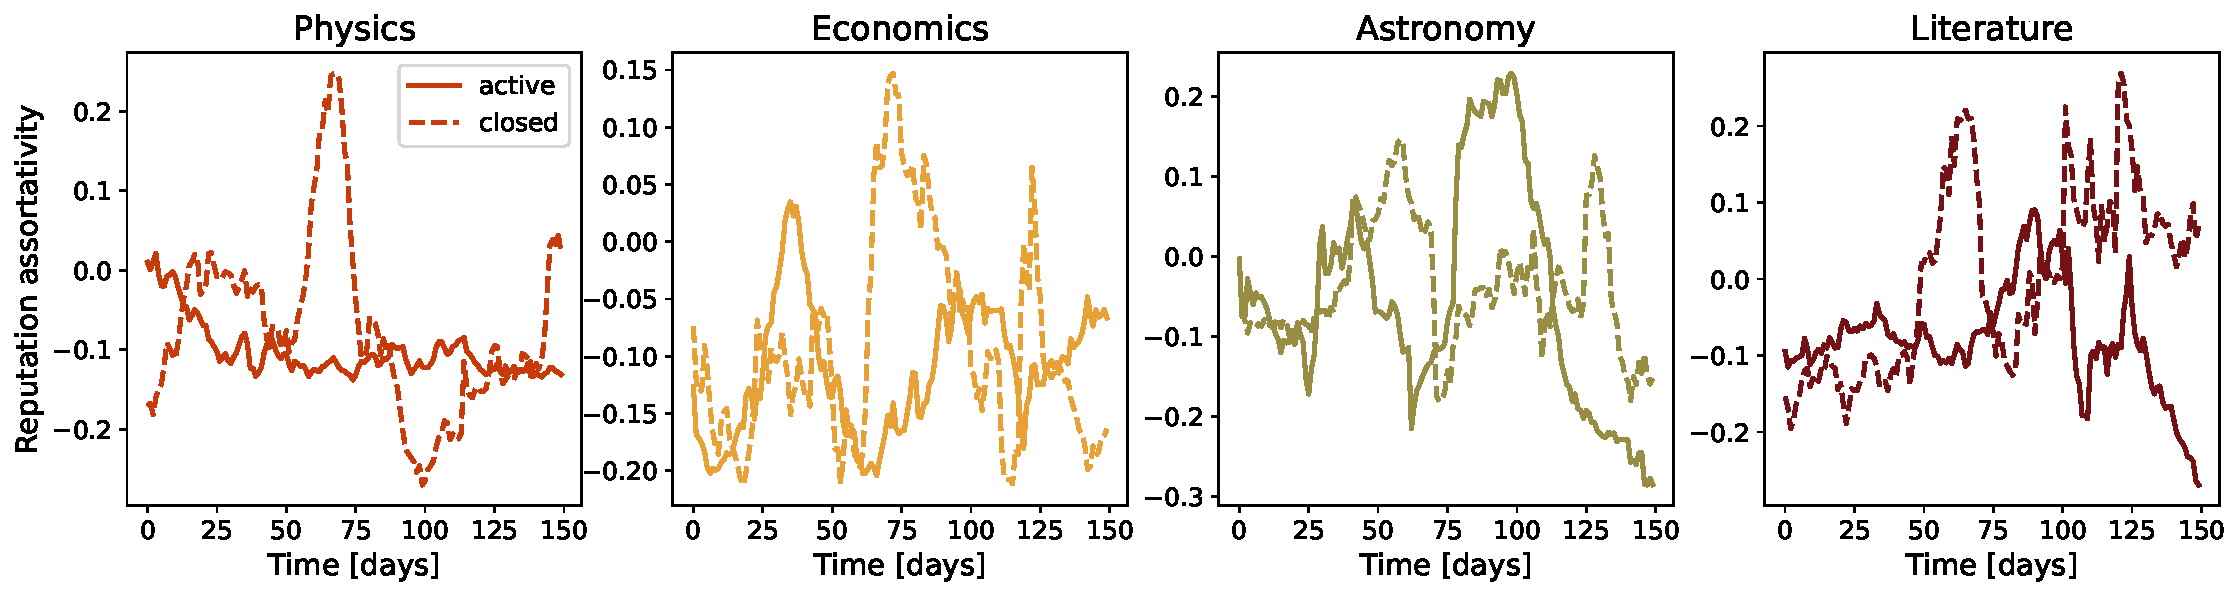
\includegraphics[width=1\linewidth]{figures/stackexchange/reputation_assortativity.pdf}
	\caption{Dynamic Reputation assortativity in the network of interactions (questions, answers, comments, unweighted, undirected network). Solid lines - active sites; dashed lines - closed sites.}
	\label{fig:dyn_rep_assort}
\end{figure}
%% posto se ovo isto gleda na mrezama mozda moze u isti section sa ova dva grafika
\\~\\
\textbf{DynRep \& Degree}
% dodacu samo korelacije kroz vreme za sad stoji samo placeholder za sliku i opis
\textbf{DynRep \& BC}
% dodacu samo korelacije kroz vreme

We continue to investigate whether the user's reputation correlates with typical network centrality measures calculated at user's node in the interaction network. As previously, we compare node's centrality in the 30 day network with the node's dynamic reputation on the last day of the period, repeat the process every day for the first six months. 
Correlation coefficient between dynamic reputation and degree in the network is very high, as expected, as most of the interactions that contributed to user's reputation are also present as links in the network. We show these results in Fig.~\ref{fig:dyn_rep_centrality}(top). However, we again see the distinction between active and closed communities where this correlation is higher in active communities, except in the first month of sliding windows. Astronomy is an exception here as well as we see that the correlations were similar in both closed and still active sites throughout observed period. 
%There are few steep drops in correlation coefficients in Economics and Literature closed sites, maybe worth further investigation.
In the bottom panels of Fig.~\ref{fig:dyn_rep_centrality} we present correlation coefficients of dynamic reputation and user's betweenness centrality in the interaction network. These corrlations are also high and most of the time higher in the later networks of active than closed communities. This is particularly interesting due to global nature of betweenness centrality measure and less obvious relation of it to user's dynamic reputation.
\begin{figure}[h!]
	\centering
	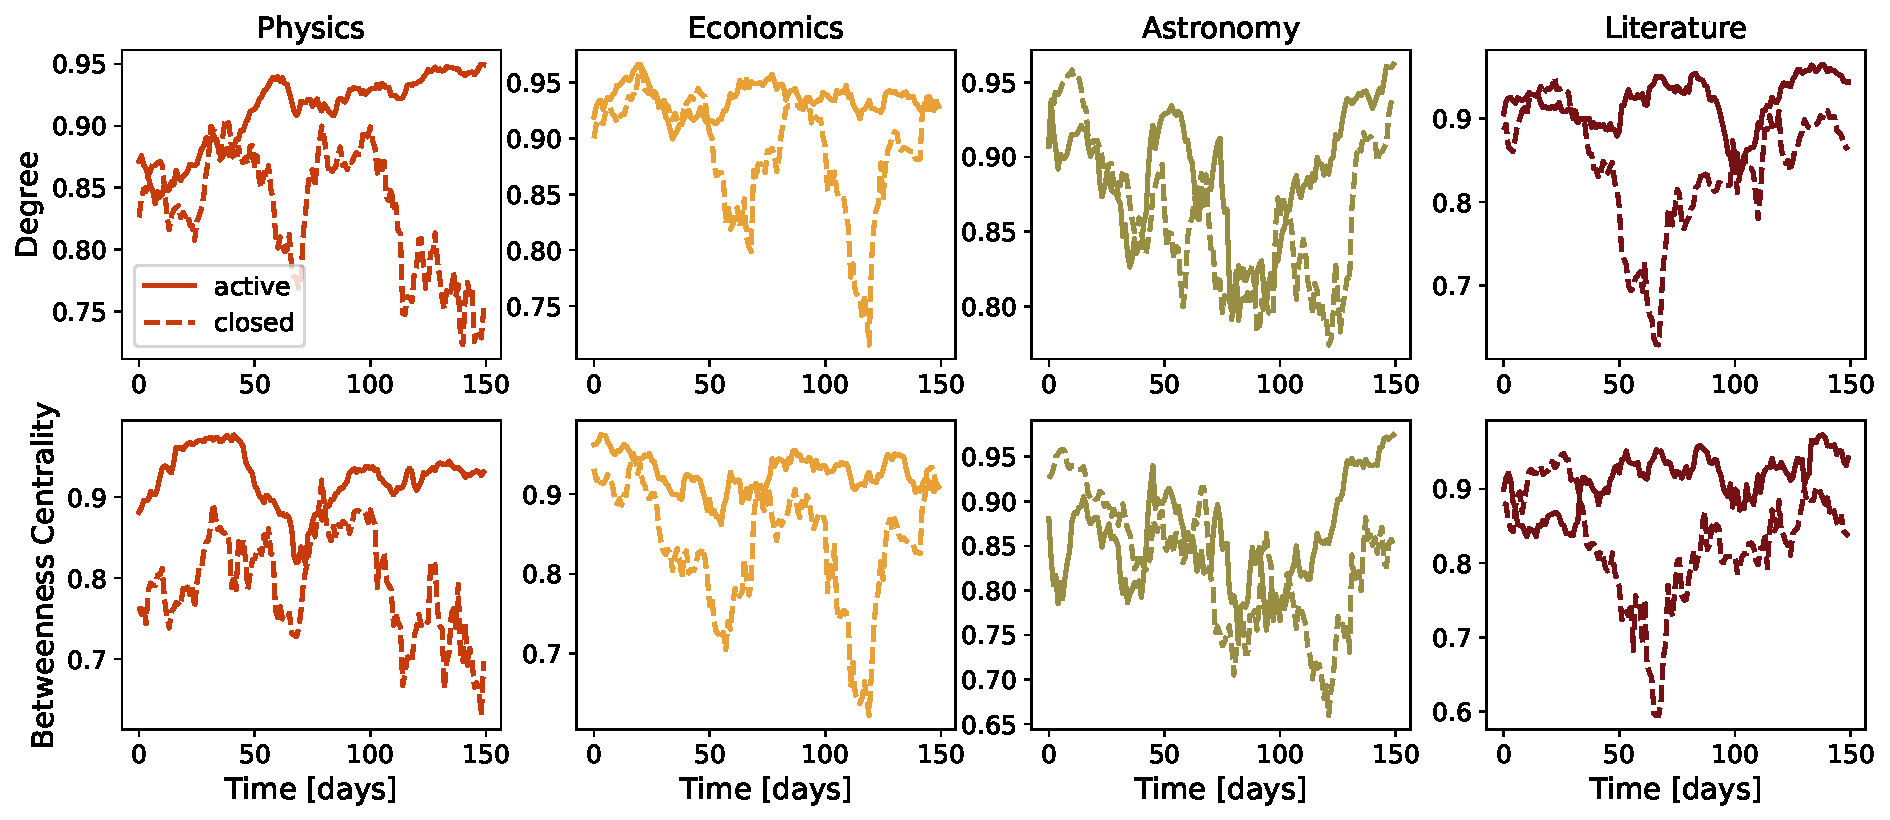
\includegraphics[width=\linewidth]{figures/stackexchange/correlations.pdf}
	\caption{Coefficient of correlation between users' Dynamic Reputation and users' network degree (top) and users's betweenness centrality (bottom). Solid lines - active sites; dashed lines - closed sites.}
	\label{fig:dyn_rep_centrality}
\end{figure}













       
